% Original bibliography embedded for a self-contained manuscript.
\begin{filecontents*}[overwrite]{Randomized_Main_embedded_refs.bib}
@book{rockafellar1998variational,
  title={Variational Analysis},
  author={Rockafellar, R Tyrrell and Wets, Roger JB},
  year={1998},
  publisher={Springer}
}
@article{deng2025smooth,
  title   = {A Smooth Approximation Framework for Weakly Convex Optimization},
  author  = {Deng, Qi and Gao, Wenzhi},
  journal = {arXiv preprint arXiv:2512.09720},
  year    = {2025}
}
@article{kong2024cost,
  title={The cost of nonconvexity in deterministic nonsmooth optimization},
  author={Kong, Siyu and Lewis, Adrian S},
  journal={Mathematics of Operations Research},
  volume={49},
  number={4},
  pages={2385--2401},
  year={2024},
  publisher={INFORMS}
}
@article{vial1983strong,
  title={Strong and weak convexity of sets and functions},
  author={Vial, Jean-Philippe},
  journal={Mathematics of Operations Research},
  volume={8},
  number={2},
  pages={231--259},
  year={1983},
  publisher={INFORMS}
}
@book{hiriart2004fundamentals,
  title={Fundamentals of Convex Analysis},
  author={Hiriart-Urruty, Jean-Baptiste and Lemar{\'e}chal, Claude},
  year={2004},
  publisher={Springer Science \& Business Media}
}
@article{drusvyatskiy2019efficiency,
  title={Efficiency of minimizing compositions of convex functions and smooth maps},
  author={Drusvyatskiy, Dmitriy and Paquette, Courtney},
  journal={Mathematical Programming},
  volume={178},
  number={1},
  pages={503--558},
  year={2019},
  publisher={Springer}
}
@article{moreau1965proximite,
  title={Proximit{\'e} et dualit{\'e} dans un espace hilbertien},
  author={Moreau, Jean-Jacques},
  journal={Bulletin de la Soci{\'e}t{\'e} math{\'e}matique de France},
  volume={93},
  pages={273--299},
  year={1965}
}
@article{davis2018stochastic,
  title={Stochastic subgradient method converges at the rate $\mathcal{O}(k^{-1/4})$  on weakly convex functions},
  author={Davis, Damek and Drusvyatskiy, Dmitriy},
  journal={arXiv preprint arXiv:1802.02988},
  year={2018}
}
@article{ghadimi2013stochastic,
  title={Stochastic first-and zeroth-order methods for nonconvex stochastic programming},
  author={Ghadimi, Saeed and Lan, Guanghui},
  journal={SIAM journal on optimization},
  volume={23},
  number={4},
  pages={2341--2368},
  year={2013},
  publisher={SIAM}
}
@inproceedings{tian2021hardness,
  title={On the hardness of computing near-approximate stationary points of Clarke regular nonsmooth nonconvex problems and certain DC programs},
  author={Tian, Lai and So, Anthony Man-Cho},
  booktitle={ICML Workshop on Beyond First-Order Methods in ML Systems},
  pages={3--6},
  year={2021}
}
@article{liao2025proximal,
  title={A proximal descent method for minimizing weakly convex optimization},
  author={Liao, Feng-Yi and Zheng, Yang},
  journal={arXiv preprint arXiv:2509.02804},
  year={2025}
}
@article{davis2019proximally,
  title={Proximally guided stochastic subgradient method for nonsmooth, nonconvex problems},
  author={Davis, Damek and Grimmer, Benjamin},
  journal={SIAM Journal on Optimization},
  volume={29},
  number={3},
  pages={1908--1930},
  year={2019},
  publisher={SIAM}
}
@article{duchi2018stochastic,
  title={Stochastic methods for composite and weakly convex optimization problems},
  author={Duchi, John C and Ruan, Feng},
  journal={SIAM Journal on Optimization},
  volume={28},
  number={4},
  pages={3229--3259},
  year={2018},
  publisher={SIAM}
}
@article{arjevani2023lower,
  title={Lower bounds for non-convex stochastic optimization},
  author={Arjevani, Yossi and Carmon, Yair and Duchi, John C and Foster, Dylan J and Srebro, Nathan and Woodworth, Blake},
  journal={Mathematical Programming},
  volume={199},
  number={1},
  pages={165--214},
  year={2023},
  publisher={Springer}
}

@book{rockafellar2009variational,
  title={Variational Analysis},
  author={Rockafellar, R Tyrrell and Wets, Roger J-B},
  volume={317},
  year={2009},
  publisher={Springer Science \& Business Media}
}

@article{nemirovsky1992information,
  title={Information-based complexity of linear operator equations},
  author={Nemirovsky, Arkadi S},
  journal={Journal of Complexity},
  volume={8},
  number={2},
  pages={153--175},
  year={1992},
  publisher={Elsevier}
}

@article{woodworth2016tight,
  title={Tight complexity bounds for optimizing composite objectives},
  author={Woodworth, Blake E and Srebro, Nati},
  journal={Advances in Neural Information Processing Systems},
  volume={29},
  year={2016}
}
@article{carmon2020lower,
  title={Lower bounds for finding stationary points {I}},
  author={Carmon, Yair and Duchi, John C and Hinder, Oliver and Sidford, Aaron},
  journal={Mathematical Programming},
  volume={184},
  number={1},
  pages={71--120},
  year={2020},
  publisher={Springer}
}
@article{CarmonEtAl2021,
  author  = {Carmon, Yair and Duchi, John C. and Hinder, Oliver and
             Sidford, Aaron},
  title   = {Lower bounds for finding stationary points {II}:
             First-order methods},
  journal = {Mathematical Programming},
  year    = {2021},
  volume  = {185},
  number  = {1--2},
  pages   = {315--355},
  doi     = {10.1007/s10107-019-01431-x}
}

@article{DavisDrusvyatskiy2019,
  author  = {Davis, Damek and Drusvyatskiy, Dmitriy},
  title   = {Stochastic model-based minimization of weakly convex functions},
  journal = {SIAM Journal on Optimization},
  year    = {2019},
  volume  = {29},
  number  = {1},
  pages   = {207--239},
  doi     = {10.1137/18M1178244}
}

@article{DiakonikolasGuzman2020,
  author  = {Diakonikolas, Jelena and Guzm{\'a}n, Crist{\'o}bal},
  title   = {Lower bounds for parallel and randomized convex optimization},
  journal = {Journal of Machine Learning Research},
  year    = {2020},
  volume  = {21},
  number  = {5},
  pages   = {1--31},
  url     = {https://jmlr.org/papers/v21/19-771.html}
}

@article{KornowskiShamir2022,
  author  = {Kornowski, Guy and Shamir, Ohad},
  title   = {Oracle complexity in nonsmooth nonconvex optimization},
  journal = {Journal of Machine Learning Research},
  year    = {2022},
  volume  = {23},
  number  = {314},
  pages   = {1--44},
  url     = {https://jmlr.org/papers/v23/21-1507.html}
}

@book{NemirovskiYudin1983,
  author    = {Nemirovsky, A. S. and Yudin, D. B.},
  title     = {Problem Complexity and Method Efficiency in Optimization},
  series    = {Wiley-Interscience Series in Discrete Mathematics},
  publisher = {John Wiley \& Sons},
  address   = {Chichester},
  year      = {1983},
  isbn      = {0-471-10345-4},
  note      = {Translated by E. R. Dawson}
}

@book{Nesterov2018,
  author    = {Nesterov, Yurii},
  title     = {Lectures on Convex Optimization},
  series    = {Springer Optimization and Its Applications},
  volume    = {137},
  edition   = {Second},
  publisher = {Springer},
  address   = {Cham},
  year      = {2018},
  isbn      = {978-3-319-91578-4},
  doi       = {10.1007/978-3-319-91578-4}
}

@article{TianSo2024,
  author  = {Tian, Lai and So, Anthony Man-Cho},
  title   = {No dimension-free deterministic algorithm computes approximate
             stationarities of {L}ipschitzians},
  journal = {Mathematical Programming},
  year    = {2024},
  volume  = {208},
  number  = {1--2},
  pages   = {51--74},
  doi     = {10.1007/s10107-023-02031-6}
}


@misc{WoodworthSrebro2017,
  author        = {Woodworth, Blake and Srebro, Nathan},
  title         = {Lower bound for randomized first order convex optimization},
  year          = {2017},
  eprint        = {1709.03594},
  archivePrefix = {arXiv},
  primaryClass  = {math.OC},
  note          = {arXiv:1709.03594},
  doi           = {10.48550/arXiv.1709.03594},
  url           = {https://arxiv.org/abs/1709.03594}
}

@inproceedings{ZhangEtAl2020,
  author    = {Zhang, Jingzhao and Lin, Hongzhou and Jegelka, Stefanie and
               Sra, Suvrit and Jadbabaie, Ali},
  title     = {Complexity of finding stationary points of nonconvex nonsmooth
               functions},
  booktitle = {Proceedings of the 37th International Conference on Machine
               Learning},
  editor    = {Daum{\'e}, III, Hal and Singh, Aarti},
  series    = {Proceedings of Machine Learning Research},
  volume    = {119},
  pages     = {11173--11182},
  publisher = {PMLR},
  year      = {2020},
  url       = {https://proceedings.mlr.press/v119/zhang20p.html}
}

\end{filecontents*}
\documentclass[11pt]{article}

% if you need to pass options to natbib, use, e.g.:
\usepackage[compress]{natbib}
\usepackage{amsmath,amssymb,amsthm}
\usepackage{color}
%\usepackage{pdfsync,enumitem,dsfont}
\usepackage[margin=1in]{geometry}
\usepackage{setspace}
\usepackage{amsthm, amsmath, amssymb, amsfonts}
\usepackage{subcaption}
\usepackage{bm}
\usepackage[dvipsnames]{xcolor}
\newcommand{\kibitz}[2]{\textcolor{#1}{#2}}
%\usepackage{lmodern}
%\usepackage[utf8]{inputenc} % allow utf-8 input
%\usepackage[T1]{fontenc}    % use 8-bit T1 fonts
%\usepackage[pdftex, colorlinks=true, citecolor=MidnightBlue, linkcolor=MidnightBlue, urlcolor=MidnightBlue]{hyperref}
\usepackage{hyperref}
\hypersetup{ colorlinks=true, citecolor=MidnightBlue, linkcolor=red!80!black, urlcolor=MidnightBlue}
\usepackage{caption}
% \usepackage{subfigure}

%\usepackage[colorlinks=false]{hyperref}       % hyperlinks
%\hypersetup{
	%	   pdfborder={0 0 0}
	%	}
\usepackage{url}            % simple URL typesetting
\usepackage{booktabs}       % professional-quality tables
\usepackage{nicefrac}       % compact symbols for 1/2, etc.
%\usepackage{microtype}      % microtypography
\usepackage{graphicx}
\usepackage{caption}
\usepackage{thm-restate}
\usepackage[export]{adjustbox}

%%%%Visual %%%
\usepackage{microtype}
\usepackage{mathpazo} % math & rm
\linespread{1.05}        % Palatino needs more leading (space between lines)
\usepackage[scaled]{helvet} % ss
\usepackage{courier} % tt
\normalfont
\usepackage[T1]{fontenc}
% \usepackage{refcheck}


%%%table 
\usepackage{threeparttable}
\allowdisplaybreaks[4] % spread setup  
\usepackage[shortlabels]{enumitem} 
\usepackage{needspace}

%% Table highlight box  
\usepackage{tikz}
\usetikzlibrary{fit}
\tikzset{%
	%highlight/.style={rectangle,blend mode = multiply,fill=blue!20,fill,rounded corners = 0.3 mm,inner sep=1pt}
	highlight/.style={rectangle,blend mode = multiply,draw=blue!90!black,thick,rounded corners = 0.3 mm,inner sep=0.5pt}
}
\newcommand{\markEle}[2]{\tikz[remember picture,overlay] \node[highlight, fit = (#1-#2-medium) (#1-#2-medium)] {};}
% tikz end
\usepackage{tcolorbox}
%equation number 
\def\O#1{\text{\ding{\the\numexpr#1+171}}} 


%Hotkey for math notations 
\newcommand{\ceil}[1]{\left\lceil #1 \right\rceil}
\newcommand{\floor}[1]{\left\lfloor #1 \right\rfloor}
\newcommand{\imply}{\Rightarrow}
\newcommand{\ifaof}{\Leftrightarrow}
\newcommand{\limto}{\rightarrow}
\newcommand{\del}{\partial}
\newcommand{\bz}{\mathbf 0}
\newcommand{\PP}{\mathbb P}
\newcommand{\QQ}{\mathbb Q}
\newcommand{\EE}{\mathbb E}
\newcommand{\R}{\mathbb R}
\newcommand{\Z}{\mathbb Z}
\newcommand{\Y}{\mathbb Y}
%\newcommand{\E}[1]{{\mathbb E}\left[ #1 \right]}
% \newcommand{\mc}{\mathcal}
\newcommand{\diff}{\mathrm{d}}
\newcommand{\eps}{\varepsilon}
\newcommand{\Let}{\triangleq}
\DeclareMathOperator{\prox}{prox}
\DeclareMathOperator{\proj}{proj}
\DeclareMathOperator{\sign}{sign}
\DeclareMathOperator{\dist}{dist}
\DeclareMathOperator*{\argmin}{argmin}
\DeclareMathOperator*{\argmax}{argmax}


\def\A{{\mathbb{A}}}
\def\B{{\mathbb{B}}}
\def\C{{\mathbb{C}}}
\def\D{{\mathbb{D}}}
% \def\E{{\mathbb{E}}}
\def\F{{\mathbb{F}}}
\def\G{{\mathbb{G}}}
\def\H{{\mathbb{H}}}
\def\I{{\delta}}
\def\J{{\mathbb{J}}}
\def\K{{\mathbb{K}}}
\def\L{{\mathbb{L}}}
\def\M{{\mathbb{M}}}
\def\N{{\mathbb{N}}}
\def\O{{\mathbb{O}}}
\def\P{{\mathbb{P}}}
\def\Q{{\mathbb{Q}}}
\def\R{{\mathbb{R}}}
\def\S{{\mathbb{S}}}
\def\T{{\mathbb{T}}}
\def\U{{\mathbb{U}}}
\def\V{{\mathbb{V}}}
\def\W{{\mathbb{W}}}
\def\X{{\mathbb{X}}}
\def\Y{{\mathbb{Y}}}
\def\Z{{\mathbb{Z}}}

\def\bA{{\mathbf{A}}}
\def\bB{{\mathbf{B}}}
\def\bC{{\mathbf{C}}}
\def\bD{{\mathbf{D}}}
\def\bE{{\mathbf{E}}}
\def\bF{{\mathbf{F}}}
\def\bG{{\mathbf{G}}}
\def\bH{{\mathbf{H}}}
\def\bI{{\mathbf{I}}}
\def\bJ{{\mathbf{J}}}
\def\bK{{\mathbf{K}}}
\def\bL{{\mathbf{L}}}
\def\bM{{\mathbf{M}}}
\def\bN{{\mathbf{N}}}
\def\bO{{\mathbf{O}}}
\def\bP{{\mathbf{P}}}
\def\bQ{{\mathbf{Q}}}
\def\bR{{\mathbf{R}}}
\def\bS{{\mathbf{S}}}
\def\bT{{\mathbf{T}}}
\def\bU{{\mathbf{U}}}
\def\bV{{\mathbf{V}}}
\def\bW{{\mathbf{W}}}
\def\bX{{\mathbf{X}}}
\def\bY{{\mathbf{Y}}}
\def\bZ{{\mathbf{Z}}}

\def\cA{{\cal A}}
\def\cB{{\cal B}}
\def\cC{{\cal C}}
\def\cD{{\cal D}}
\def\cE{{\cal E}}
\def\cF{{\cal F}}
\def\cG{{\cal G}}
\def\cH{{\cal H}}
\def\cI{{\cal I}}
\def\cJ{{\cal J}}
\def\cK{{\cal K}}
\def\cL{{\cal L}}
\def\cM{{\cal M}}
\def\cN{{\cal N}}
\def\cO{{\cal O}}
\def\cP{{\cal P}}
\def\cQ{{\cal Q}}
\def\cR{{\cal R}}
\def\cS{{\cal S}}
\def\cT{{\cal T}}
\def\cU{{\cal U}}
\def\cV{{\cal V}}
\def\cW{{\cal W}}
\def\cX{{\cal X}}
\def\cY{{\cal Y}}
\def\cZ{{\cal Z}}

\def\a{\bm{a}}
\def\b{\bm{b}}
\def\c{\bm{c}}
\def\d{\bm{d}}
\def\e{\bm{e}}
\def\f{\bm{f}}
\def\g{\bm{g}}
\def\h{\bm{h}}
\def\i{\bm{i}}
\def\j{\bm{j}}
\def\k{\bm{k}}
\def\l{\bm{l}}
\def\m{\bm{m}}
\def\n{\bm{n}}
\def\o{\bm{o}}
\def\p{\bm{p}}
\def\q{\bm{q}}
\def\r{\bm{r}}
\def\s{\bm{s}}
\def\t{\bm{t}}
\def\u{\bm{u}}
\def\v{\bm{v}}
\def\w{\bm{w}}
\def\x{\bm{x}}
\def\y{\bm{y}}
\def\z{\bm{z}}
\def\bz{{\mathbf 0}}
\def\lbd{{\lambda}}
\def\1{{\mathbf 1}}
\def\intm{{\rm int}}
\def\bmu{\bm{\mu}}
\def\blam{\bm{\lambda}}

\DeclareMathOperator{\cl}{cl}
\DeclareMathOperator{\dom}{dom}
\DeclareMathOperator{\kl}{KL}
\DeclareMathOperator{\rank}{rank}
% for def over equal
\newcommand{\defequal}{\overset{\text{\tiny{def}}}{=}}
\newcommand{\commentColor}{blue!90!black}
%Topology related
% \DeclareMathOperator{\dim}{dim}
\DeclareMathOperator{\codim}{codim}
\DeclareMathOperator{\rand}{rand}
\DeclareMathOperator{\aff}{aff}
\DeclareMathOperator{\spann}{span}
\DeclareMathOperator{\inter}{int}
\DeclareMathOperator{\rint}{rint}
\DeclareMathOperator{\bd}{bd}
\DeclareMathOperator{\rbd}{rbd}



%thm environment 
\usepackage{thmtools}
\renewcommand{\qedsymbol}{$\blacksquare$}
%\declaretheoremstyle[qed=$\square$,parent=section]{definitionwithend}
\declaretheoremstyle[parent=section]{definitionwithend}
\declaretheorem[style=definitionwithend]{corollary}
\declaretheorem[style=definitionwithend]{theorem}
\declaretheorem[style=definitionwithend]{proposition}
\declaretheorem[style=definitionwithend]{definition}
\declaretheorem[style=definitionwithend]{assumption}
\declaretheorem[style=definitionwithend]{example}
\declaretheorem[style=definitionwithend]{remark}
\declaretheorem[style=definitionwithend]{question}
\declaretheorem[style=definitionwithend]{lemma}
\declaretheorem[style=definitionwithend]{fact} 
\declaretheorem[style=definitionwithend]{observation} 

\newcommand{\Jiajin}[1]{{\scriptsize\textbf{\color{black}[Jiajin: #1]}}}


% Compatibility additions required by the weakly convex manuscript.
% They do not alter the visual style inherited from the template.
\usepackage{mathtools}
\usepackage{pifont}
\usepackage[nameinlink]{cleveref}
\usepackage[titletoc]{appendix}
\setlength{\emergencystretch}{3em}

\declaretheorem[style=definitionwithend]{condition}
\declaretheorem[style=definitionwithend]{claim}

\crefname{assumption}{Assumption}{Assumptions}
\crefname{lemma}{Lemma}{Lemmas}
\crefname{theorem}{Theorem}{Theorems}
\crefname{corollary}{Corollary}{Corollaries}
\crefname{proposition}{Proposition}{Propositions}
\crefname{condition}{Condition}{Conditions}
\crefname{claim}{Claim}{Claims}
\crefname{figure}{Figure}{Figures}
\crefname{remark}{Remark}{Remarks}
\crefname{section}{Section}{Sections}
\crefname{example}{Example}{Examples}
\crefname{definition}{Definition}{Definitions}
\crefname{table}{Table}{Tables}
\crefname{equation}{}{}
\crefname{enumi}{}{}
\crefname{appendix}{Appendix}{Appendices}
\Crefname{appendix}{Appendix}{Appendices}

\usepackage{tikz}
\usetikzlibrary{arrows.meta,positioning}

% Manuscript-specific notation not supplied by the template.
\def\mc{\mathcal}
\def\sA{{\mathsf{A}}}
\def\sZ{{\mathsf{Z}}}
\DeclareMathOperator{\supp}{supp}
\DeclareMathOperator{\Lip}{Lip}
\DeclareMathOperator{\zr}{zr}
\newcommand{\norm}[1]{\left\lVert #1\right\rVert}
\newcommand{\Siyu}[1]{\kibitz{orange}{[Siyu: #1]}}
\title{Optimal {\color{black}Randomized} Oracle Complexity for \\Weakly Convex Optimization}

\date{\today}
\author{%
Jiajin Li \qquad Siyu Pan\\[0.75em]
Sauder School of Business,\\
The University of British Columbia\\[0.5em]
\small \texttt{\{jiajin.li,siyu.pan\}@sauder.ubc.ca}
}

% Unique PDF destinations preserve links across section-reset theorem counters.
\hypersetup{hypertexnames=false,
  pdftitle={Optimal Randomized Oracle Complexity for Weakly Convex Optimization},
  pdfauthor={Jiajin Li and Siyu Pan}}
\begin{document}
\maketitle

% {\color{orange}Siyu: Here is GPT's view: don''t use the term ``optimal'' since the term “optimal” must be interpreted relative to a fixed stationarity
% measure, oracle model, and output convention. \citet{DavisDrusvyatskiy2019,liao2025proximal,kong2024cost} use different settings. Personally, I don't think it will cause big trouble.
% }


\begingroup
\color{black}
\begin{abstract}
We study the oracle complexity of finding $\epsilon$-stationary points
of globally $G$-Lipschitz, $\rho$-weakly convex functions with initial
gap at most $\Delta$. Stationarity is measured by the gradient of the
Moreau envelope, and the oracle returns both the function value and
the full subdifferential. We establish the optimal randomized complexity
$\Theta(\rho G^2\Delta/\epsilon^4)$ whenever
$0<\epsilon<\min\{G,\sqrt{\rho\Delta}\}$ and
$\Delta\leq(G^2/\rho)\exp(G^2/(200\epsilon^2))$,
with universal constants at
every positive confidence level.
Our proof develops an abstract lower-bound framework that converts
layered locality of the complete oracle and a Moreau stationarity
barrier into a lower bound on one fixed instance for each randomized
algorithm. The framework permits unrestricted queries and arbitrary
outputs. We verify its conditions using tilted convex blocks coupled
into overlapping chains, whose information propagates through a
constant-width diagonal filtration. A Lipschitz majorant and a radial
modification preserve global regularity and the stationarity barrier
while preventing distant queries from revealing the hidden frame.
The $\epsilon^{-4}$ dependence therefore persists without oracle noise,
even when the algorithm randomizes its queries.
\end{abstract}

\endgroup


\begingroup
\color{black}
\section{Introduction}
\label{sec:introduction}
The oracle complexity of finding stationary points in nonconvex
optimization is well understood in the smooth setting.
First-order methods achieve the optimal complexity
$\Theta(\epsilon^{-2})$ \citep{CarmonEtAl2021,carmon2020lower},
whereas stochastic first-order methods require
$\Theta(\epsilon^{-4})$ oracle queries
\citep{arjevani2023lower,ghadimi2013stochastic}.

The current complexity picture for weakly convex optimization is less
conclusive. Weakly convex functions encompass smooth nonconvex and
convex-composite objectives
\citep{vial1983strong,drusvyatskiy2019efficiency}.
For this class, stochastic subgradient methods attain an
$\mathcal O(\epsilon^{-4})$ oracle complexity for finding an
$\epsilon$-stationary point, with stationarity measured by the
gradient of the Moreau envelope
\citep{DavisDrusvyatskiy2019,davis2019proximally,davis2018stochastic}.
This naturally raises the following question:
\begin{center}
\setlength{\fboxsep}{10pt}
\fbox{\parbox{0.9\textwidth}{\centering\bfseries
Can deterministic first-order methods break the
$\epsilon^{-4}$ barrier?}}
\end{center}

We show that the $\epsilon^{-4}$ dependence is already necessary
for deterministic first-order methods. Randomizing the queries
does not improve this dependence, even with exact first-order
oracles. The additional $\epsilon^{-2}$ factor therefore reflects
the nonsmooth geometry of the problem class.

Specifically, we study the oracle complexity of the weakly convex
optimization problem
\begin{equation}
\label{eq:prob}
\min_{\x\in\R^d} f(\x),
\tag{P}
\end{equation}
where $f:\R^d\to\R$ is globally $G$-Lipschitz,
$\rho$-weakly convex for some $\rho>0$, and possibly nonsmooth.
We assume that $f(\bz)-\inf f\leq\Delta$.
Let $f_\lambda$ denote the Moreau envelope of $f$, with
$\lambda=1/(2\rho)$. A point $\x$ is $\epsilon$-stationary if
$\|\nabla f_\lambda(\x)\|\leq\epsilon$.
We adopt a first-order oracle that returns both the function value
and the \emph{full subdifferential} at every query point.
This stronger oracle ensures that our lower bound does not rely
on an unfavorable choice of subgradient by the oracle.

\subsection{Our Results and Techniques}
We first state an informal version of our main lower bound.
\begin{theorem}[Informal]
In the principal parameter regime, the randomized first-order
oracle complexity of finding an $\epsilon$-stationary point with
probability at least $1-\nu$ is
\[
 \Omega\!\left(\frac{\rho G^2\Delta}{\epsilon^4}\right),
\]
with universal implied constants for every $\nu\in[0,1)$.
\end{theorem}
This lower bound matches a deterministic upper bound in its dependence
on all problem parameters. Theorem~\ref{thm:main} states the precise
parameter conditions and the resulting optimal complexity.

We develop a generalized zero-chain framework for proving randomized
oracle lower bounds. The framework organizes hidden directions into
layers and separates five requirements: global regularity, robust
locality of the complete oracle, a terminal Moreau stationarity barrier,
an initial-gap bound, and exterior control. Theorem~\ref{thm:abstract-randomized} converts
these requirements into a lower bound determined by the number of
layers. Its conclusion holds on one fixed instance for the whole finite
trajectory and a prescribed arbitrary output, with the instance chosen
independently of the realized private seed.

Our hard instance verifies these requirements using two ingredients.
First, we extend the classical zero-chain construction
\citep{CarmonEtAl2021} to the full-subdifferential oracle.
We construct a tilted max-affine convex block whose entire
subdifferential satisfies a setwise zero-chain property. Strictly
ordered intercepts ensure that, when unrevealed coordinates are
sufficiently small, only the first unrevealed facet can become active.

Second, we use this convex block to construct a weakly convex hard
instance consisting of multiple coupled and overlapping chains.
A diagonal filtration organizes the coordinate directions across
blocks into layers, each containing at most five directions; see
Figure~\ref{fig:overlapping-relay}. Under the small-projection condition,
the function value and full subdifferential depend only on the next
revealed prefix. This gives a constant-width analogue of the classical
zero chain with $\Theta(MN)$ layers.

A Lipschitz majorant controls the global Lipschitz constant
independently of the number of blocks. A radial modification makes
sufficiently distant oracle responses independent of the hidden
frame while preserving the stationarity barrier for the final
function's Moreau envelope. These properties allow us to apply the
abstract framework to arbitrary randomized algorithms and derive
the lower bound after scaling the construction to the prescribed
values of $G$, $\rho$, and $\Delta$.
\endgroup

\begin{figure}[t]
\centering
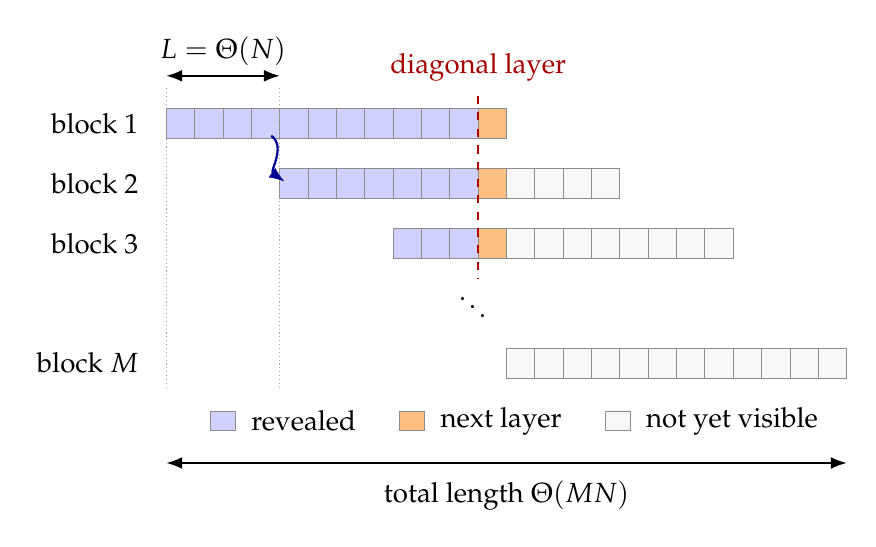
\begin{tikzpicture}[
    x=0.36cm,
    y=0.76cm,
    cell/.style={
      draw=black!45,
      line width=0.35pt,
      minimum width=0.36cm,
      minimum height=0.38cm,
      inner sep=0pt
    },
    revealed/.style={cell,fill=blue!18},
    frontier/.style={cell,fill=orange!50},
    hidden/.style={cell,fill=black!3},
    >=Latex
]
\def\BlockLength{12}
\def\RelayDelay{4}
\def\CurrentLevel{10}
\def\TotalDepth{24}

% The first three block rows.
\foreach \m in {1,2,3} {
  \pgfmathtruncatemacro{\shift}{(\m-1)*\RelayDelay}
  \pgfmathtruncatemacro{\yy}{1-\m}
  \node[anchor=east] at (-0.65,\yy+0.25) {block \(\m\)};
  \foreach \j in {1,...,\BlockLength} {
    \pgfmathtruncatemacro{\lev}{\shift+\j-1}
    \pgfmathtruncatemacro{\nextlevel}{\CurrentLevel+1}
    \ifnum\lev<\nextlevel
      \node[revealed] at (\lev+0.5,\yy+0.25) {};
    \else
      \ifnum\lev=\nextlevel
        \node[frontier] at (\lev+0.5,\yy+0.25) {};
      \else
        \node[hidden] at (\lev+0.5,\yy+0.25) {};
      \fi
    \fi
  }
}

% Omitted intermediate blocks and the terminal block.
\node at (10.8,-2.68) {\(\ddots\)};
\node[anchor=east] at (-0.65,-3.75) {block \(M\)};
\foreach \j in {1,...,\BlockLength} {
  \pgfmathtruncatemacro{\xx}{12+\j-1}
  \node[hidden] at (\xx+0.5,-3.75) {};
}

% Delay between two consecutive block starts.
\draw[<->,line width=0.6pt]
  (0,1.05)--(\RelayDelay,1.05)
  node[midway,above] {\(L=\Theta(N)\)};
\draw[densely dotted,black!35] (0,0.84)--(0,-4.15);
\draw[densely dotted,black!35]
  (\RelayDelay,0.84)--(\RelayDelay,-4.15);

% Relay to the next block before the first block is exhausted.
\draw[-{Latex[length=2mm]},blue!58!black,line width=0.8pt]
  (\RelayDelay-0.30,0.05)
  to[out=-36,in=145]
  (\RelayDelay+0.18,-0.72);

% One diagonal layer in the shifted display.
\pgfmathtruncatemacro{\NextLevel}{\CurrentLevel+1}
\draw[dashed,red!68!black,line width=0.75pt]
  (\NextLevel,0.72)--(\NextLevel,-2.35);
\node[anchor=south,text=red!65!black]
  at (\NextLevel,0.79) {diagonal layer};

% Legend entries are positioned by their rendered text widths.
\node[revealed,minimum width=0.32cm,minimum height=0.25cm]
  (legend-revealed) at (2,-4.72) {};
\node[anchor=west,right=2pt of legend-revealed]
  (legend-revealed-text) {revealed};
\node[frontier,minimum width=0.32cm,minimum height=0.25cm,
      right=12pt of legend-revealed-text] (legend-next) {};
\node[anchor=west,right=2pt of legend-next]
  (legend-next-text) {next layer};
\node[hidden,minimum width=0.32cm,minimum height=0.25cm,
      right=12pt of legend-next-text] (legend-hidden) {};
\node[anchor=west,right=2pt of legend-hidden] {not yet visible};

% Total serialized length.
\draw[<->,draw=black,line width=0.6pt]
  (0,-5.42)--(\TotalDepth,-5.42);
\node[anchor=north] at (12,-5.55) {total length \(\Theta(MN)\)};
\end{tikzpicture}
\caption{Schematic of the overlapping relay across blocks.}
\label{fig:overlapping-relay}
\end{figure}

\paragraph{Notation.}
Bold lowercase letters such as $\x,\y$ denote vectors.  Scalar coordinates are written without boldface; for example, $x_i$ is a scalar coordinate.  We write $\|\cdot\|$ for the Euclidean norm. For a positive integer $T$, we use the shorthand notation $[T] := \{1,\ldots,T\}$ to denote the index set of the first $T$ positive integers. Additionally, we denote $[0]=\varnothing$ for convenience. For integers \(d'\ge d\), we denote the set of column-orthonormal matrices by $
        \mbox{O}(d',d)
        :=
        \{\mathbf U\in\mathbb R^{d'\times d}\mid
        \mathbf U^\top\mathbf U=\bI_d\}$. 
        We use the convention that \(\inf\varnothing=+\infty\).
        For $\a\in\R^d$, write $[\a]_+:=(\max\{a_1,0\},\ldots,\max\{a_d,0\})$. Fix $M,N\in\N$. For $n\in[N]$, let $\e_n$ denote the $n$-th standard basis vector of $\R^N$; for $m\in[M]$ and $n\in[N]$, let $\e_{mn}$ denote the corresponding
standard basis vector of the ambient space $\R^{MN}$. 
The zero vector in \(\R^d\) is denoted by \(\bz_d\); when the ambient
dimension is clear from context, we simply write \(\bz\). We denote the \(d\times d\) identity matrix by \(\bI_d\). We write $\supp(\a)$ for the support of a vector $\a$.
        

\begingroup
\color{black}
\paragraph{Structure of the paper.}
Section~\ref{sec:pre} introduces the function class, stationarity
measure, oracle, and algorithmic complexity model.
Section~\ref{sec:framework} states the main result, develops
the abstract framework, and completes the random-rotation and scaling
arguments that reduce the main theorem to hard-instance properties.
Sections~\ref{sec:construction} and~\ref{sec:verification}
construct the coupled blocks and verify those properties.
Section~\ref{sec:close} concludes the paper.
The appendices give the isometric embedding identities, numerical
checks, matching upper bound, and auxiliary convex certificates.
\endgroup




\section{Preliminaries}
\label{sec:pre}
This section introduces the function class, stationarity measure,
and full-subdifferential oracle. We then define the class of
randomized first-order algorithms and the associated oracle complexity.
\begin{definition}[Function Class]
Suppose that \(G,\rho>0\) {\color{black}and} {\color{black}\(\Delta\geq0\)}. We define \(\mathcal F(G,\rho,\Delta)\)
as the union, over dimensions \(d\in\N\), of the classes of functions
\(f:\R^d\to\R\) satisfying the following properties:
\begin{enumerate}[label=(\roman*)]
 \item (\(\rho\)-weak convexity) \(f\) is \(\rho\)-weakly convex.
 % i.e., $f+\frac{\rho}{2}\norm{\cdot}^2$ is convex. 
 \item ($G$-Lipschitz continuity) $f$ is $G$-Lipschitz, i.e., for all $\x,\y\in \R^d$, 
 $$
 |f(\x)-f(\y)|\leq G\|\x-\y\|. 
 $$
 \item (Initial gap)  The initialization satisfies $f(\bz)-\inf_{\x\in\R^d} f(\x)\leq\Delta$.
\end{enumerate}
\end{definition}

{We introduce the stationarity measure used throughout the paper.}
\begin{definition}[$\epsilon$-stationary point]
\label{def:stationary}
Let $\lambda=1/(2\rho)$, and define the Moreau envelope of $f$ by
\[
 f_\lambda(\x):=\min_{\z\in\R^d}
 \left\{f(\z)+\frac{1}{2\lambda}\|\x-\z\|^2\right\}.
\]
Given $\epsilon>0$, a point $\x\in\R^d$ is an
$\epsilon$-stationary point of problem~\eqref{eq:prob} if
$\|\nabla f_\lambda(\x)\|\leq\epsilon$.
\end{definition}

{We consider the generalized first-order oracle (FO), denoted by
$\mathbb O_f(\x)$.}
\begin{definition}[{\color{black}First-order Oracle}]
For each query point \(\x\in\R^d\) and each admissible \(f\), the {\color{black}first-order} oracle returns both the function value and the full subdifferential set, i.e.,
$\mathbb{O}_f(\x) \coloneqq (f(\x),\partial f(\x))$. 
\end{definition}

\begingroup
\color{black}
For finite weakly convex functions on $\R^d$, the Fr\'echet,
limiting, and Clarke subdifferentials coincide and are nonempty,
compact, and convex \citep{rockafellar2009variational}.
Functions in the stated class are called admissible.
Let $\mathcal K_d$ denote the space of nonempty compact convex
subsets of $\R^d$, equipped with the Borel $\sigma$-algebra
induced by the Hausdorff metric.

\begin{definition}[Randomized first-order algorithm]
\label{def:randomized-algorithm}
A randomized first-order algorithm $\sA$ is specified by a private
seed $\xi_{\sA}\sim\operatorname{Unif}[0,1]$, drawn independently
of $f$, and, in each dimension $d$, Borel measurable maps
\[
 \Gamma_{d,t}:
 [0,1]\times(\R\times\mathcal K_d)^t\longrightarrow\R^d,
 \qquad t\geq1.
\]
For every admissible $f:\R^d\to\R$, the algorithm starts from
$\sA^{(0)}[f]=\bz$ and generates its queries according to
\[
 \sA^{(t)}[f]=\Gamma_{d,t}\left(
 \xi_{\sA},
 \bigl(\mathbb O_f(\sA^{(s)}[f])\bigr)_{s=0}^{t-1}
 \right),\qquad t\geq1.
\]
The decision rules may depend on the problem parameters.
We denote the class of such algorithms by $\mathcal A_{\rand}$.
\end{definition}

\begin{definition}[Oracle complexity]
\label{def:complexity-algorithm-class}
For $\epsilon>0$ and $\nu\in[0,1)$, the oracle complexity
of a nonempty algorithm class $\cA\subseteq\cA_{\rand}$
on a nonempty admissible function class $\cF$ is
\[
\begin{aligned}
 \cT_{\epsilon,\nu}(\cA,\cF)
 :=\inf_{\sA\in\cA}\sup_{f\in\cF}
 \inf\bigl\{t\in\N_0:\;&
 \P_{\xi_{\sA}}\bigl(
 \|\nabla f_\lambda(\sA^{(t)}[f])\|\leq\epsilon
 \bigr)\geq1-\nu\bigr\},
\end{aligned}
\]
where $\lambda=1/(2\rho)$.
\end{definition}

Here $\N_0:=\{0,1,2,\ldots\}$ and $\inf\varnothing:=+\infty$.
The output $\sA^{(t)}[f]$ is formed after $t$ oracle replies
and need not itself be queried. In particular, $t=0$
allows returning the initial point $\bz$.
\endgroup


\begingroup
\color{black}
\section{Main Results and a Generalized Zero-Chain Framework}
\label{sec:framework}

\subsection{Main Results}
\label{subsec:main-results}
\begin{theorem}[Randomized oracle complexity]
\label{thm:main}
\label{thm:rand}
Let $G,\rho>0$ and $\nu\in[0,1)$. Suppose that
\[
 0<\epsilon<\min\!\left\{G,\sqrt{\rho\Delta}\right\},
 \qquad
 \Delta\leq\frac{G^2}{\rho}
       \exp\!\left(\frac{G^2}{200\epsilon^2}\right).
\]
There are universal constants $c,C>0$ such that, for the exact
full-subdifferential oracle,
\[
 c\frac{\rho G^2\Delta}{\epsilon^4}
 \leq\cT_{\epsilon,\nu}
       (\cA_{\rand},\cF(G,\rho,\Delta))
 \leq C\frac{\rho G^2\Delta}{\epsilon^4}.
\]
The upper bound is attained by a deterministic algorithm.
The constants are independent of the confidence parameter $\nu$.
\end{theorem}


\begin{remark}[Arbitrary outputs]
The lower bounds also apply when, after at most $T$ oracle calls on
every run, the algorithm returns an arbitrary Borel measurable function
of its private seed and transcript. The output is included as one more
candidate in the same small-projection event and need not be queried.
The hard function is fixed independently of the realized private seed.
This statement concerns a bound on the number of calls on every run.
\end{remark}

\begin{remark}[Role of the weak convexity modulus]
For every finite oracle horizon $T$, one can choose a finite weak
convexity modulus $\rho(T)$ for which $T$ queries are insufficient
\citep{tian2021hardness}. Accordingly, the unbounded union
$\bigcup_{\rho>0}\cF(G,\rho,\Delta)$ has no uniform finite-time
complexity guarantee; controlling $\rho$ is essential.
\end{remark}

\subsection{Generalized zero chains}
\label{subsec:abstract-framework}

We formulate five properties of a normalized hard instance.
A coordinate filtration records the directions revealed by successive
oracle responses. To handle randomized algorithms, the oracle identity
and stationarity bound must remain valid when unrevealed projections
are sufficiently small.

Call a pair of integers $(M,N)$ admissible if
\begin{equation}
 N\ge256,\qquad 2\le M\le2^{8N}.
 \label{eq:normalized-admissible}
\end{equation}
Fix an admissible pair, put $K=MN$, and let $T\ge1$ be an integer
oracle-call horizon. We use the same block coordinates throughout:
\[
 \z=(\z^1,\ldots,\z^M),\qquad
 \z^m=(z_{m1},\ldots,z_{mN}),\qquad m\in[M].
\]
Here $z_{mn}$ is coordinate $n\in[N]$ of block $m\in[M]$,
and $\e_{mn}$ is its standard basis vector.
Let $I_{-1}=\varnothing$ and, for $0\le t<T$, choose index sets with
\[
 I_{t-1}\subseteq I_t\subsetneq[M]\times[N],
 \qquad |I_t\setminus I_{t-1}|\le5.
\]
The associated coordinate filtration is
$V_t:=\operatorname{span}\{\e_{mn}:(m,n)\in I_t\}$.

Index the columns of an orthonormal frame
$U=(u_{mn})_{(m,n)\in[M]\times[N]}\in\operatorname O(d,K)$
in lexicographic order, and write $U_{I_t}$ for the columns
indexed by $I_t$. Set
\[
 q_t(U,\x):=\max_{(m,n)\notin I_t}|\langle u_{mn},\x\rangle|.
\]
Thus $q_t$ measures the largest projection onto an unrevealed
direction. We interpret $\operatorname O(d,0)$ as the singleton
empty frame.

\Needspace{7\baselineskip}
\begin{condition}[Normalized hard-instance properties]
\label{cond:abstract-framework}
Fix $B,\eta>0$. For each $d\ge K$, consider a family
$\{h_U:\R^d\to\R\}_{U\in\operatorname O(d,K)}$ satisfying
the following conditions uniformly in $U$.
\begin{enumerate}[label=\textnormal{(C\arabic*)},leftmargin=*]
\item\label{cond:framework-regularity}
\emph{Regularity.}
The function $h_U$ is finite, bounded below, $1$-Lipschitz,
and $1$-weakly convex.

\item\label{cond:framework-locality}
\emph{Robust oracle locality.}
For each $0\le t<T$, there is a Borel map
$\mathcal R_{d,t}:\R^d\times\operatorname O(d,|I_t|)
\to\R\times\mathcal K_d$ such that
\begin{equation}
 \|\x\|\le B,\quad q_{t-1}(U,\x)<\eta
 \quad\Longrightarrow\quad
 \mathbb O_{h_U}(\x)=\mathcal R_{d,t}(\x,U_{I_t}).
 \label{eq:framework-locality}
\end{equation}

\item\label{cond:framework-barrier}
\emph{Terminal stationarity barrier.}
The horizon satisfies $T\ge MN/16$, and
\begin{equation}
 \|\x\|\le B,\quad q_{T-1}(U,\x)<\eta
 \quad\Longrightarrow\quad
 \|\nabla(h_U)_{1/2}(\x)\|>\frac1{32\sqrt N}.
 \label{eq:framework-barrier}
\end{equation}

\item\label{cond:framework-gap}
\emph{Initial gap.}
$h_U(\bz)-\inf h_U\le3M/N$.

\item\label{cond:framework-exterior}
\emph{Exterior control.}
There is a Borel map
$\mathcal R_{d,\mathrm{out}}:\R^d\to\R\times\mathcal K_d$,
independent of $U$, such that
\begin{equation}
 \|\x\|>B
 \quad\Longrightarrow\quad
 \left\{
 \begin{aligned}
 \mathbb O_{h_U}(\x)&=\mathcal R_{d,\mathrm{out}}(\x),\\
 \|\nabla(h_U)_{1/2}(\x)\|&=1.
 \end{aligned}
 \right.
 \label{eq:framework-exterior}
\end{equation}
\end{enumerate}
The response maps are common to all frames and defined on their
entire domains, including arguments that fail the small-projection
condition. For each $d$, the maps
$(U,\x)\mapsto\mathbb O_{h_U}(\x)$ and
$(U,\x)\mapsto\nabla(h_U)_{1/2}(\x)$ are jointly Borel measurable.
\end{condition}

Condition \textnormal{(C2)} restricts the complete oracle to the
exposed directions and the next layer, while allowing a known radial
component. Both stationarity estimates apply to the final function
$h_U$; \textnormal{(C5)} covers queries outside the ball.

\subsection{A randomized rotation theorem}
\label{subsec:randomized-rotation}

The robust oracle identity limits how many hidden directions each
reply can reveal. To apply this restriction to arbitrary randomized
queries, we first simulate the algorithm using only the directions
revealed so far. Conditional on this information and the private seed,
the next query is fixed while the remaining directions are random.
Small-projection estimates then identify the simulated transcript
with the true one. Averaging over the rotation gives a single hard
instance, independent of the realized seed.
\begin{theorem}[Randomized rotation]
\label{thm:abstract-randomized}
Suppose that Condition~\ref{cond:abstract-framework} holds.
Fix $\delta\in(0,1)$ and an ambient dimension satisfying
\begin{equation}
 d\geq K+2+
 \left\lceil\frac{4K(T+1)B^2}{\delta\eta^2}\right\rceil.
 \label{eq:framework-dimension}
\end{equation}
For every randomized first-order algorithm in $\R^d$ and every
Borel output rule $\widehat\x$ based on its private seed and
first $T$ oracle replies, there exists a fixed frame
$U_\star\in\operatorname O(d,K)$ such that, with probability
at least $1-\delta$ over the private seed,
\[
 \|\nabla(h_{U_\star})_{1/2}(\x)\|>\frac1{32\sqrt N}
 \quad\text{for every }\x\in
 \{\x^0,\ldots,\x^{T-1},\widehat\x\}.
\]
Here $\x^0,\ldots,\x^{T-1}$ are the queries on $h_{U_\star}$.
The frame is independent of the realized seed. The output rule is
defined for every seed and transcript of length $T$; its output
need not be queried or bounded. Borel stopping rules bounded by $T$
on every run are also allowed.
\end{theorem}

\begin{proof}
Draw $U$ uniformly from $\operatorname O(d,K)$, independently of
the private seed $\xi_{\sA}$.

\emph{Simulation.}
At time $t$, form the simulated query $\widetilde\x^t$ from the
seed and preceding simulated replies, and return
\[
 \widetilde{\mathbb O}_t=
 \begin{cases}
 \mathcal R_{d,t}(\widetilde\x^t,U_{I_t}),
       &\|\widetilde\x^t\|\le B,\\
 \mathcal R_{d,\mathrm{out}}(\widetilde\x^t),
       &\|\widetilde\x^t\|>B.
 \end{cases}
\]
Thus $\widetilde\x^t$ depends only on
$(\xi_{\sA},U_{I_{t-1}})$, and the simulated output
$\widetilde{\widehat\x}$ depends only on
$(\xi_{\sA},U_{I_{T-1}})$.
The globally defined response maps make this a Borel simulation on
every seed and frame, even when a projection test fails. Revealing
columns to the simulator gives the algorithm only the displayed reply.

\emph{Small projections and coupling.}
Conditional on $(\xi_{\sA},U_{I_{t-1}})$, the query is fixed and
every unexposed column is uniform on the sphere in the remaining
orthogonal complement. Its second moment gives, for $(m,n)\notin I_{t-1}$,
\[
 \mathbb P\!\left(
  \|\widetilde\x^t\|\le B,\quad
  |\langle u_{mn},\widetilde\x^t\rangle|>\eta/2
  \,\middle|\,\xi_{\sA},U_{I_{t-1}}
 \right)
 \le\frac{4B^2}{(d-K)\eta^2}.
\]
The same estimate holds for the output, conditional on
$(\xi_{\sA},U_{I_{T-1}})$.
There are at most $K(T+1)$ tests. Hence
\eqref{eq:framework-dimension} and a union bound give an event
$E$ of probability at least $1-\delta$ on which
\[
 \begin{aligned}
 \|\widetilde\x^t\|\le B
 &\ \Longrightarrow\ q_{t-1}(U,\widetilde\x^t)\le\eta/2
 &&(0\le t<T),\\
 \|\widetilde{\widehat\x}\|\le B
 &\ \Longrightarrow\ q_{T-1}(U,\widetilde{\widehat\x})\le\eta/2.
 \end{aligned}
\]
The estimates condition only on the seed and exposed columns, not
on earlier successful tests. On $E$, conditions \textnormal{(C2)}
and \textnormal{(C5)} identify each simulated reply with the actual
oracle response. Induction therefore identifies all queries and
the output.

\emph{A fixed hard instance.}
Let $E_{\mathrm{act}}$ denote the same projection conditions for
the actual queries and output. The coupling gives
$E\subseteq E_{\mathrm{act}}$, so averaging over $U$ yields a
fixed frame $U_\star$ satisfying
\begin{equation}
 \mathbb P_{\xi_{\sA}}
 (E_{\mathrm{act}}\mid U=U_\star)\ge1-\delta.
 \label{eq:rotation-transcript}
\end{equation}
Joint measurability justifies this averaging. The frame may depend
on the algorithm and output rule, but not on the realized seed.
The argument so far uses only \textnormal{(C2)} and the exterior
oracle identity in \textnormal{(C5)}, and applies to any finite
coordinate index set.

On $E_{\mathrm{act}}$, every bounded candidate satisfies
$q_{T-1}(U_\star,\x)<\eta$, since
$I_{t-1}\subseteq I_{T-1}$. Condition \textnormal{(C3)} gives
the required stationarity bound there; \textnormal{(C5)} gives
gradient norm one at every candidate outside the ball.
For a Borel stopping rule bounded by $T$, retain its output and
pad unused calls with queries at the origin.
\end{proof}

\Needspace{8\baselineskip}
For $0<\epsilon\le1/(32\sqrt N)$ and $\nu\in[0,1)$, take
$\delta=(1-\nu)/2$ and
$\widehat\x=\sA^{(T)}[h_{U_\star}]$.
The theorem gives one function on which each candidate indexed
by $0,\ldots,T$ has success probability at most
$\delta<1-\nu$. By \textnormal{(C1)} and \textnormal{(C4)},
this function belongs to
$\cF(1,1,3M/N)$. Hence
\begin{equation}
 \cT_{\epsilon,\nu}
 \bigl(\cA_{\rand},\cF(1,1,3M/N)\bigr)
 \geq T+1.
 \label{eq:framework-complexity}
\end{equation}
The confidence level affects the sufficient dimension, not the
number of layers.

The classical coordinate chain corresponds to width one.
Our coupled construction has a diagonal filtration of width
at most five and a horizon $T=\Theta(MN)$.
Subsection~\ref{subsec:scaling-reduction} completes the scaling and
parameter argument. The construction and verification of the required
families are deferred to Sections~\ref{sec:construction}
and~\ref{sec:verification}.

\endgroup




\subsection{Scaling and proof of the main theorem}
\label{subsec:scaling-reduction}
\label{sec:proof-main}

The two chain lengths control different quantities. The stationarity
barrier is of order $G/\sqrt N$, so we take
$N\asymp G^2/\epsilon^2$. The initial gap is of order
$G^2M/(\rho N)$, which permits $M\asymp\rho\Delta N/G^2$.
The resulting horizon has order
\[
 MN\asymp\frac{\rho G^2\Delta}{\epsilon^4}.
\]
We now justify this scaling and check the integer and admissibility
constraints.
\begin{lemma}[Scaling]
\label{lem:scaling}
Suppose that $\{h_U\}$ satisfies
Condition~\ref{cond:abstract-framework}. Fix $G,\rho>0$ and
$\delta\in(0,1)$, and define
\[
 f_U(\x):=\frac{G^2}{\rho}
 h_U\!\left(\frac\rho G\x\right).
\]
Then $f_U$ is $G$-Lipschitz and $\rho$-weakly convex, with
\[
 f_U(\bz)-\inf f_U\le\frac{3G^2M}{\rho N}.
\]
Under the dimension bound in \eqref{eq:framework-dimension},
for every randomized algorithm and Borel output after $T$ replies,
there is a fixed $U_\star$ such that, with probability at least
$1-\delta$, all its first $T$ queries and its output satisfy
\[
 \|\nabla(f_{U_\star})_{1/(2\rho)}(\x)\|
 >\frac G{32\sqrt N}.
\]
\end{lemma}

\begin{proof}
Put $\z=(\rho/G)\x$.
The regularity and gap claims follow from \textnormal{(C1)} and
\textnormal{(C4)}. Changing variables in the proximal minimization
and using the subdifferential chain rule gives
\begin{equation}
 \mathbb O_{f_U}(\x)
 =\left(\frac{G^2}{\rho}h_U(\z),\ G\partial h_U(\z)\right),
 \qquad
 \nabla(f_U)_{1/(2\rho)}(\x)
 =G\nabla(h_U)_{1/2}(\z).
 \label{newrand:actual-scaling}
\end{equation}
To simulate an algorithm on $f_U$ using the oracle of $h_U$,
query at $\z=(\rho/G)\x$ and transform each returned pair by
$(v,S)\mapsto((G^2/\rho)v,GS)$. Use the same private seed and
scale the output by $\rho/G$. These transformations are Borel
measurable and preserve the number of calls.
Theorem~\ref{thm:abstract-randomized} applied to the simulated
algorithm gives a fixed frame and the simultaneous stationarity
bound. The gradient identity in \eqref{newrand:actual-scaling}
then gives the stated conclusion for $f_U$.
\end{proof}

The next theorem completes the parameter choice using only the
five conditions. Sections~\ref{sec:construction}
and~\ref{sec:verification} will construct and verify the required
normalized family.

\begin{theorem}[Scaling reduction]
\label{thm:scaling-reduction}
\label{newrand:main-range}
Suppose that, for every admissible $(M,N)$, there are a family
$\{h_U\}$, an integer horizon $T$, a coordinate filtration,
and $B,\eta>0$ satisfying Condition~\ref{cond:abstract-framework}.
If $G,\rho,\Delta,\epsilon>0$ satisfy
\[
 \frac{G^2}{\epsilon^2}\ge2^{18},\qquad
 \frac{\rho\Delta}{\epsilon^2}\ge2^{18},\qquad
 \Delta\le\frac{G^2}{\rho}
       \exp\!\left(\frac{G^2}{200\epsilon^2}\right),
\]
then, for every $\nu\in[0,1)$,
\begin{equation}
 \cT_{\epsilon,\nu}
 \bigl(\cA_{\rand},\cF(G,\rho,\Delta)\bigr)
 \ge 2^{-29}\frac{\rho G^2\Delta}{\epsilon^4}.
 \label{newrand:count}
\end{equation}
The bound also holds for arbitrary Borel outputs when the number
of oracle calls is bounded on every run.
\end{theorem}

\begin{proof}
Write $b=G^2/\epsilon^2$, $r=\rho\Delta/G^2$, and
$s=br=\rho\Delta/\epsilon^2$. Choose
\begin{equation}
 N=\left\lfloor\frac b{1024}\right\rfloor,
 \qquad M=\left\lfloor\frac{rN}{3}\right\rfloor,
 \qquad
 f_U(\x)=\frac{G^2}{\rho}
 h_U\!\left(\frac\rho G\x\right).
 \label{newrand:scaling}
\end{equation}
Since $b,s\ge2^{18}$, the floor estimates give
\[
 N\ge256,\qquad N\ge\frac b{2048},\qquad
 \frac{rN}{3}\ge\frac s{6144}>2,\qquad
 M\ge\frac{rN}{6}\ge2.
\]
To check $M\le2^{8N}$, use $\ln2\ge2/3$ and
$\log_2N\le N/32$ for $N\ge256$.
Since $r\le e^{b/200}$ and $b<1024(N+1)\le1028N$,
\[
 \log_2M\le\log_2r+\log_2N
 \le\frac{3b}{400}+\frac N{32}<8N.
\]
Thus $(M,N)$ is admissible.
Lemma~\ref{lem:scaling} shows that $f_U$ is $G$-Lipschitz and
$\rho$-weakly convex, with
\[
 f_U(\bz)-\inf f_U
 \le\frac{G^2}{\rho}\frac{3M}{N}\le\Delta.
\]
Apply that lemma with $\delta=(1-\nu)/2$ and a sufficient finite
dimension. For every algorithm and its chosen output rule,
one fixed instance makes all its first $T$ queries and its output
satisfy
\[
 \|\nabla(f_U)_{1/(2\rho)}(\x)\|
 >\frac G{32\sqrt N}\ge\epsilon
\]
simultaneously with probability at least $(1+\nu)/2>\nu$.
The last inequality follows from $N\le b/1024$.
By \textnormal{(C3)},
\[
 T\ge\frac{MN}{16}
 \ge\frac{rN^2}{96}
 \ge\frac{b^2r}{96\cdot2^{22}}\ge\frac{b^2r}{2^{29}}
 =2^{-29}\frac{\rho G^2\Delta}{\epsilon^4}.
\]
Taking the output to be $\sA^{(T)}[f_U]$ gives simultaneous
failure at every candidate indexed by $0,\ldots,T$.
As in \eqref{eq:framework-complexity}, this proves
\eqref{newrand:count} for the stated trajectory complexity.
\end{proof}

The scaling reduction treats the regime in which both
$b=G^2/\epsilon^2$ and $s=\rho\Delta/\epsilon^2$ are large.
When only $b$ is large, a single convex chain gives an
$\Omega(b)$ bound, which suffices because $s$ is bounded.
When $b$ is bounded, the assumed gap range also bounds the target
$bs$, and it remains only to rule out a zero-call guarantee.
The two convex certificates used below are proved in
Appendix~\ref{app:principal-completion}.
\begin{proof}[Proof of Theorem~\ref{thm:main}]
Put
\[
 b=\frac{G^2}{\epsilon^2},\qquad
 s=\frac{\rho\Delta}{\epsilon^2},\qquad
 r=\frac sb,\qquad B_0=2^{18}.
\]
The assumptions give $b>1$, $s>1$, and $r\le e^{b/200}$;
the target complexity is $bs$.

\emph{Case 1: $b,s\ge B_0$.}
Lemma~\ref{lem:normalized-instance}, proved in
Subsection~\ref{subsec:verify-normalized}, verifies the five conditions
for every admissible pair.
Theorem~\ref{thm:scaling-reduction} therefore gives the lower bound
$2^{-29}bs$.

\emph{Case 2: $b\ge B_0$ and $1<s<B_0$.}
Lemma~\ref{lem:principal-bridge} supplies an auxiliary convex
family in $\cF(G,\rho,\epsilon^2/\rho)\subseteq\cF(G,\rho,\Delta)$,
with
\[
 K=\lfloor b/8\rfloor,\qquad T=\lfloor K/8\rfloor.
\]
Its prefix and exterior oracle identities allow the transcript
argument in the proof of Theorem~\ref{thm:abstract-randomized}
to be applied with coordinate index set $[K]$.
Choose $\delta=(1-\nu)/2$ and $d$ as in
\eqref{eq:framework-dimension}, using the lemma's radius and
tolerance. Equation~\eqref{eq:rotation-transcript} then gives
one fixed frame on which all bounded queries and the bounded
output have small unrevealed projections, with probability
at least $1-\delta$. The lemma's strict Moreau bound exceeds
$\epsilon$ at these candidates and at every candidate outside
the ball. Thus all candidates fail simultaneously on this event.
Since $K\ge b/10$,
\[
 \cT_{\epsilon,\nu}\ge T+1>\frac K8
 \ge\frac b{80}\ge\frac{bs}{80B_0}.
\]
The same argument includes any prescribed Borel output.

\emph{Case 3: $1<b<B_0$.}
Here
\[
 bs=b^2r\le Q_\star:=B_0^2e^{B_0/200}<\infty.
\]
It suffices to exclude zero-query algorithms. By
Lemma~\ref{lem:one-query}, there is an admissible cone family
$\{f_u\}_{\|u\|=1}$ whose $\epsilon$-stationary set is
$\overline B(au,h)$, with $0<h/a\le3/4$.
Draw $u$ uniformly on the unit sphere. For any fixed $\x\ne\bz$,
membership in this ball implies
\[
 \left\langle u,\frac\x{\|\x\|}\right\rangle
 \ge\frac{\|\x\|^2+a^2-h^2}{2a\|\x\|}
 \ge\frac{\sqrt{a^2-h^2}}a\ge\frac{\sqrt7}{4}.
\]
The spherical second moment and Markov's inequality give
\[
 \mathbb P_u\{\x\in\overline B(au,h)\}
 \le\frac{16}{7d}.
\]
The probability is zero at $\x=\bz$. A zero-query output $X$
is independent of $u$, so averaging over $X$ gives the same bound.
Choose $d>16/[7(1-\nu)]$ and average over $u$ to obtain a fixed
instance on which $X$ fails with probability greater than $\nu$.
Thus $\cT_{\epsilon,\nu}\ge1\ge Q_\star^{-1}bs$.

The three cases establish the lower bound with the universal constant
\[
 c=\min\{2^{-29},(80B_0)^{-1},Q_\star^{-1}\}>0.
\]
Each case covers arbitrary Borel outputs with a bound on the
number of oracle calls on every run. The instance is fixed
independently of the realized private seed; the confidence level
affects only the sufficient ambient dimension.

For the upper bound, the assumptions imply
$\epsilon^2\le\min\{G^2,\rho\Delta\}$.
Proposition~\ref{prop:matching-upper} gives a deterministic algorithm
using at most $C\rho G^2\Delta/\epsilon^4$ oracle calls, with success
probability one. This completes the proof.
\end{proof}

The remaining sections construct a family satisfying the hypotheses
of Theorem~\ref{thm:scaling-reduction} and verify those hypotheses.


\begingroup
\color{black}
\section{The construction of our hard instance}
\label{sec:construction}
\label{newrand:extension}
Fix integers $M\ge2$ and $N\ge256$, and put $K=MN$.
We write $\z=(\z^1,\ldots,\z^M)$, where
$\z^m=(z_{m1},\ldots,z_{mN})\in\R^N$.
We first construct a convex tilted max-affine block whose entire
subdifferential satisfies a setwise zero-chain property.
We then couple $M$ copies so that progress in one block activates
the next block before the preceding block is complete.
The diagonal filtration in Section~\ref{sec:verification} will
describe the information revealed by these overlapping chains.

\subsection{A tilted max-affine block} 
For $m\in[M]$ and $n\in[N]$, define
\begin{equation}
 c_{mn}:=1+\frac{K-(m-1)N-n+1}{32(K+1)}.
 \label{newrand:fan}
\end{equation}
These intercepts lie in $(1,33/32)$ and decrease strictly in the
lexicographic order of $(m,n)$. For each $m\in[M]$, define
\[
 \phi_m(\bm u)
 :=\max\left\{0,\max_{n\in[N]}
       \left(c_{mn}-\frac N8u_n\right)\right\},
 \qquad \bm u\in\R^N.
\]
This block adapts the max-affine constructions used for nonsmooth
convex lower bounds~\citep{WoodworthSrebro2017,DiakonikolasGuzman2020}.
When the unrevealed coordinates are zero, the strictly ordered
intercepts ensure that only the first unrevealed affine piece can
be active.

\begin{lemma}
\label{lem:tilted-block-locality}
For every {$m\in[M]$ and} \(k\in\{0,\ldots,N-1\}\), we have 
\[
 \bm{u}\in\operatorname{span}\{\e_1,\ldots,\e_k\}
 \quad\Longrightarrow\quad
 \partial\phi_{m}(\bm{u})
 \subseteq
 \operatorname{span}\{\e_1,\ldots,
\e_{k+1}\}.
\]
\end{lemma}
\begin{proof}
If $u_n=0$ for $n>k$, the values of the corresponding affine
pieces are $c_{m,k+1}>\cdots>c_{mN}$. Thus no piece indexed by
$n>k+1$ is active. Every subgradient is a convex combination of
the active slopes, which belong to
$\{0,-(N/8)\e_1,\ldots,-(N/8)\e_{k+1}\}$.
\end{proof}

The tilted max-affine block therefore enforces the required setwise
zero-chain property within a single block, but it can hide only \(N\)
coordinates. Taking \(M\) independent copies does not produce an
\(MN\)-step lower bound, since {an algorithm} could explore
all blocks in parallel. We therefore couple consecutive blocks so that
block \(m\) can become active only after sufficient progress has been made
in block \(m-1\). This coupling converts the parallel blockwise chains into
a constant-width diagonal chain and supplies the additional factor \(M\)
in the oracle lower bound.

\subsection{Coupling the tilted blocks}
\label{subsec:block-coupling}
To impose a sequential dependence across blocks, we
use a smooth function to transmit progress from block \(m\) to block
\(m+1\).  Define 
\[
 q(t)
 :=
 \begin{cases}
  0, & t\leq 0,\\
  3t^2-2t^3, & 0<t<1,\\
  1, & t\geq 1.
 \end{cases}
\]
Define the smooth progress function \(\psi:\R^N\to[0,1]\) by
\[
 \psi(\bm{u})
 :=
 \frac{1}{N}\sum_{n=1}^N
 q\left(\frac{N}{4}u_n{-\theta}\right),\qquad {\theta:=\frac1{64N}.}
\]
The value \(\psi(\z^m)\) records the progress made within block \(m\).
Since \(q({-\theta})=q'({-\theta})=0\), an unrevealed coordinate \(z_{mn}=0\)
contributes zero both to \(\psi(\z^m)\) and to the \(n\)-th component of
\(\nabla\psi(\z^m)\).

We use this progress function to couple consecutive blocks.
For $m\in[M]$, define
\begin{equation}
 p_m(\z):=q\left(\frac{4\psi(\z^m)-1}{3}\right),
 \qquad p_0:=1.
 \label{newrand:gate}
\end{equation}
The quantity $p_m(\z)$ vanishes whenever $\psi(\z^m)\le1/4$.
We then define the block scores
\[
 \sigma_m(\z):=\phi_m(\z^m)+p_{m-1}(\z)-\frac54,
 \qquad m\in[M],
\]
and write $\boldsymbol\sigma(\z)=(\sigma_1(\z),\ldots,\sigma_M(\z))$.
Here $p_{m-1}(\z)$ transmits progress from block $m-1$ to
block $m$, while $p_0=1$ initializes the first block.

We combine the block scores and progress functions to define
the coupled function
\begin{equation}
 f_0(\z):=\frac2N\left(
    \|[\boldsymbol\sigma(\z)]_+\|
    -2\sum_{m=1}^M\psi(\z^m)\right).
 \label{eq:hard}
\end{equation}
The positive part suppresses blocks with negative scores.
The subtracted term rewards progress within each block; its
coefficient ensures that this decrease is not canceled by the
activation of the next block. We verify this sign property in
the subdifferential formula below.

\begin{remark}[Overlapping activation across blocks]
\label{rem:block-relay}
The score $\sigma_m$ implements a relay between consecutive blocks.
Consider an unstarted block $m\ge2$, so that $\z^m=0$.
Since $\phi_m(0)=c_{m1}\in(1,33/32)$, we have
\[
 \begin{aligned}
 \psi(\z^{m-1})\le\tfrac14
 &\quad\Longrightarrow\quad \sigma_m(\z)<0,\\
 \psi(\z^{m-1})\ge\tfrac12
 &\quad\Longrightarrow\quad \sigma_m(\z)>0.
 \end{aligned}
\]
Thus, the next block can become active before the preceding
block is complete. Activation nevertheless requires progress
in sufficiently many coordinates: since $0\le q\le1$ and
$q(-\theta)=0$,
\[
 \psi(\z^{m-1})
 \le\frac{|\operatorname{supp}(\z^{m-1})|}{N}.
\]
Hence an unstarted block cannot become active unless more than
$\lfloor N/4\rfloor$ coordinates in the preceding block are nonzero.
\end{remark}

The Lipschitz constant of $f_0$ may grow with $M$.
To obtain a uniform bound, we define its least $2$-Lipschitz
majorant by
\begin{equation}
 F(\z):=\sup_{\y\in\R^K}
       \{f_0(\y)-2\|\z-\y\|\}.
 \label{newrand:majorant}
\end{equation}
Proposition~\ref{prop:regularity} shows that $F$ is finite-valued,
bounded below, $2$-Lipschitz, and $9/2$-weakly convex.
The later oracle and stationarity estimates are proved for
this majorant, taking account of every maximizing point in
\eqref{newrand:majorant}.

\endgroup


\begingroup
\color{black}
\section{Verification of the abstract conditions}
\label{sec:verification}
We now verify the five conditions of the abstract framework in
Subsection~\ref{subsec:abstract-framework}. We establish global regularity,
introduce the diagonal filtration and prove robust oracle locality,
derive a stationarity barrier, and bound the initial gap.
The radial modification preserves the barrier for the final function
and supplies the required exterior control.

\subsection{Lipschitz continuity and weak convexity}
\label{subsec:regularity}
We show that $F$ is finite-valued, bounded below, $2$-Lipschitz,
and $9/2$-weakly convex. The main observation is that a variational
representation separates the convex block terms from the smooth
terms, each of which depends on a single block.

Let $\mc W:=\{\bm w\in\R_+^M:\|\bm w\|\le1\}$ and set
$w_{M+1}:=0$.
\begin{lemma}[Variational representation]
\label{lem:max-representation}
For every $\z\in\R^K$,
\[
 f_0(\z)=\max_{\bm w\in\mc W}F_{\bm w}(\z),
\]
where
\begin{equation}
 F_{\bm w}(\z):=\frac2N\Biggl[
 w_1+\sum_{m=1}^M\Bigl(
 w_m\bigl(\phi_m(\z^m)-\tfrac54\bigr)
 +w_{m+1}p_m(\z)-2\psi(\z^m)\Bigr)\Biggr].
 \label{eq:Fw}
\end{equation}
\end{lemma}
\begin{proof}
For every $\a\in\R^M$,
$\|[\a]_+\|=\max_{\bm w\in\mc W}\langle\bm w,\a\rangle$.
Apply this identity to $\boldsymbol\sigma(\z)$ and use
\[
 \sum_{m=1}^M w_mp_{m-1}(\z)
 =w_1+\sum_{m=1}^M w_{m+1}p_m(\z),
\]
which follows from $p_0=1$ and $w_{M+1}=0$.
Substitution in \eqref{eq:hard} gives \eqref{eq:Fw}.
\end{proof}

We first record the estimates on the progress function.
\begin{lemma}[Regularity of the progress function]
\label{lem:progress-regularity}
For every $\bm u\in\R^N$,
\[
 0\le\psi(\bm u)\le1,\qquad
 \|\nabla\psi(\bm u)\|\le\frac{3\sqrt N}{8},\qquad
 \operatorname{Lip}(\nabla\psi)\le\frac{3N}{8}.
\]
\end{lemma}
\begin{proof}
On $0<t<1$, we have $q'(t)=6t(1-t)$ and $q''(t)=6-12t$.
The one-sided first derivatives agree at both junctions, so
$q\in C^1(\R)$, with
$0\le q\le1$, $0\le q'\le3/2$, and
$\operatorname{Lip}(q')\le6$.
Since $\psi$ is an average of values of $q$, it lies in $[0,1]$.
The chain rule gives
\[
 \nabla\psi(\bm u)
 =\frac14\bigl(q'(Nu_n/4-\theta)\bigr)_{n=1}^N.
\]
The bound on $q'$ gives $\|\nabla\psi(\bm u)\|\le3\sqrt N/8$.
For any $\bm u,\bm v\in\R^N$, its Lipschitz bound gives
\[
 \|\nabla\psi(\bm u)-\nabla\psi(\bm v)\|^2
 \le\sum_{n=1}^N\left(\frac{3N}{8}|u_n-v_n|\right)^2
 =\frac{9N^2}{64}\|\bm u-\bm v\|^2.\qedhere
\]
\end{proof}

We next establish a weak-convexity bound independent of $M$ and $N$.
\begin{lemma}[Weak convexity of the coupled function]
\label{lem:coupled-curvature}
The function $f_0$ is $9/2$-weakly convex.
\end{lemma}
\begin{proof}
Write $h(s)=q((4s-1)/3)$. Then $0\le h'\le2$ and
$\operatorname{Lip}(h')\le32/3$.
For $\omega\in[0,1]$, consider the smooth block term
\[
 G_\omega(\bm u)=\omega h(\psi(\bm u))-2\psi(\bm u).
\]
Its gradient is
$\nabla G_\omega=(\omega h'(\psi)-2)\nabla\psi$.
Using $|\omega h'(\psi)-2|\le2$ and
Lemma~\ref{lem:progress-regularity}, the product and chain rules
for Lipschitz bounds give
\[
 \operatorname{Lip}(\nabla G_\omega)
 \le 2\frac{3N}{8}
    +\frac{32}{3}\left(\frac{3\sqrt N}{8}\right)^2
 =\frac{9N}{4}.
\]
Thus every $G_\omega$ is $9N/4$-weakly convex.
In \eqref{eq:Fw}, these terms occupy disjoint blocks, so their
sum has the same weak-convexity bound. Adding the convex terms
$w_m\phi_m$ and multiplying by $2/N$ gives the common bound
$9/2$ for every $F_{\bm w}$. Their maximum $f_0$ inherits this bound.
\end{proof}



\begin{proposition}[Regularity of the majorant]
\label{prop:regularity}
The function $F$ is finite-valued, bounded below, $2$-Lipschitz,
and $\rho_0$-weakly convex. Moreover, $f_0$ is coordinatewise
nonincreasing, and
\[
 \operatorname{Lip}\left(\frac2N\|[\boldsymbol\sigma(\cdot)]_+\|\right)
 \le c_N:=\frac14+\frac3{2\sqrt N}\le\frac{11}{32}.
\]
The supremum in \eqref{newrand:majorant} is attained, and its
maximizing points stay in a bounded set when $\z$ ranges over
a bounded set.
\end{proposition}
\begin{proof}
We first establish monotonicity and growth bounds for $f_0$.
Each $\phi_m$ is coordinatewise nonincreasing.
For $h(s)=q((4s-1)/3)$, the smooth term of block $m$ in
\eqref{eq:Fw} has gradient
\[
 \bigl(w_{m+1}h'(\psi(\z^m))-2\bigr)\nabla\psi(\z^m)\le0
\]
coordinatewise. Hence each $F_{\bm w}$, and therefore $f_0$,
is coordinatewise nonincreasing.

For the Lipschitz bound on the positive-score term, use
\[
 \frac2N\|[\boldsymbol\sigma(\z)]_+\|
 =\max_{\bm w\in\mc W}\frac2N\sum_m w_m\sigma_m(\z).
\]
Since the blocks are orthogonal, the weighted fan terms have
Lipschitz constant at most $\|\bm w\|/4\le1/4$.
Also $\|\nabla p_m\|\le2\|\nabla\psi\|\le3\sqrt N/4$,
so the weighted activation terms have Lipschitz constant at most
$3\|\bm w\|/(2\sqrt N)\le3/(2\sqrt N)$.
Taking the maximum proves the bound $c_N$.
Since $0\le\psi\le1$, we also have
\begin{equation}
 f_0(\z)\ge-\frac{4M}{N}=:m_0.
 \label{eq:lower_f}
\end{equation}

To control the supremum defining $F$, put $u=(9/N)\mathbf1_K$.
The bounds $p_m\le1$ and $c_{mn}<9/8$ give
$[\sigma_m(\y)]_+\le\phi_m(\y^m)
\le(N/8)\|(u^m-\y^m)_+\|$. Consequently,
\begin{equation}
 f_0(\y)\le\frac2N\|[\boldsymbol\sigma(\y)]_+\|
 \le\frac14\|(u-\y)_+\|.
 \label{newrand:growth}
\end{equation}
It follows that
\[
 f_0(\y)-2\|\z-\y\|
 \le\frac14\|u-\z\|-\frac74\|\z-\y\|.
\]
The right side tends to $-\infty$ as $\|\y\|\to\infty$,
uniformly for bounded $\z$. Continuity now gives finiteness,
attainment, and the asserted bound on maximizing points.

Each function $\z\mapsto f_0(\y)-2\|\z-\y\|$ is
$2$-Lipschitz, so their finite supremum $F$ is $2$-Lipschitz.
Finally, the translated representation
\[
 F(\z)=\sup_v\{f_0(\z+v)-2\|v\|\}
\]
expresses $F$ as a supremum of functions with common
weak-convexity modulus $\rho_0$. It inherits that modulus,
and $F\ge f_0\ge m_0$ proves boundedness below.
\end{proof}

\subsection{A generalized zero-chain property} 
\label{sec:locality} 
Let
$
 {\ell:=\left\lfloor\frac N4\right\rfloor.}
$ 
We assign to each coordinate direction \(\e_{mn}\) the level
\[
 \operatorname{lev}(m,n):=(m-1){\ell}+n-1.
\]
For every \(r\geq0\), define the \(r\)-th diagonal layer by
\[
 \mathcal E_r
 :=
 \operatorname{span}
 \left\{
   \e_{mn}:
   \operatorname{lev}(m,n)=r
 \right\}.
\]
Set $I_{-1}=\varnothing$ and
$I_t:=\{(m,n)\in[M]\times[N]:\operatorname{lev}(m,n)\le t\}$
for $t\ge0$. The corresponding diagonal filtration is 
\begin{equation}
\label{newrand:filtration}
 {V}_{-1}:=\{0\},
 \quad \text{and} \quad
 {V}_t
 :=
 \bigoplus_{r=0}^t\mathcal E_r
 =
 \operatorname{span}
 \left\{
   \e_{mn}:
   \operatorname{lev}(m,n)\leq t
 \right\},
 \qquad  \forall t\geq0.
\end{equation}
Thus \({V}_t\) contains all coordinate directions up to level \(t\)
in the staggered ordering.  The following lemma makes precise that this
filtration has constant-width increments. 

\begin{lemma}[Width of the diagonal filtration]
\label{lem:diagonal-width}
For every \(t\geq-1\),
\[
 {V}_{t+1}
 =
 {V}_t\oplus\mathcal E_{t+1},
 \quad \text{and} \quad
 \dim\left(
   {V}_{t+1}/{V}_t
 \right)
 =
 \dim(\mathcal E_{t+1})
 \leq{5}.
\]
\end{lemma}
\begin{proof}[Proof of Lemma~\ref{lem:diagonal-width}]
The direct-sum identity follows from the definition of the filtration.
To bound the dimension of a layer, fix \(r\geq0\).  The equality
\(\operatorname{lev}(m,n)=r\) implies
$
 n=r-(m-1){\ell}+1\in[N],
$
and hence
\[
 r-N+1
 \leq
 (m-1){\ell}
 \leq
 r.
\]
Thus the admissible values of \((m-1){\ell}\) lie in an interval of length
\(N-1\) and are separated by \({\ell}\).  Therefore,
\[
 \dim(\mathcal E_r)
 \leq
 1+\left\lfloor\frac{N-1}{{\ell}}\right\rfloor
 =
 \left\lceil\frac N{{\ell}}\right\rceil.
\]
Since {\(N\geq256\)},
we have $
 {\ell}
 \geq
 {\tfrac N4-1}
 \geq
 {\tfrac N5}.
$
Therefore \(\lceil N/{\ell}\rceil\leq{5}\).
\end{proof}
The preceding lemma controls the total number of coordinate directions in
each diagonal layer. 
We next compute the full subdifferential. Write
$h(s)=q((4s-1)/3)$ and define
\[
 a_m(\bm w,\z):=2-w_{m+1}h'(\psi(\z^m))\in[0,2].
\]
This nonnegative coefficient ensures that the progress term and
the active fan slopes point in the same coordinatewise direction.


\begin{lemma}[Characterization of the subdifferential]
\label{lem:full-subdiff}
Let
$
 R(\z):=\norm{[\boldsymbol{\sigma}(\z)]_+}$ and $
 \mathcal I(\z)
 :=
 \operatorname*{argmax}_{\bm{w}\in\mathcal W}
 \langle \bm{w},\boldsymbol{\sigma}(\z)\rangle.
$
Then
\begin{equation}
 \partial{f_0}(\z)
 =
 \operatorname{conv}
 \left(
   \bigcup_{\bm{w}\in\mathcal I(\z)}
   \mathcal G(\bm{w},\z)
 \right),
 \label{eq:full-subdiff}
\end{equation}
where \(\mathcal G(\bm{w},\z)\) is the nonempty compact convex set of vectors
\(\g=(\g^1,\ldots,\g^M)\) satisfying for all $ m\in[M]$,
\begin{equation}
 \g^m
 =
 \frac2N
 \left(
   w_m\bm{u}_m
   -
   a_m(\bm{w}{,\z})\nabla\psi(\z^m)
 \right),
 \qquad
 \bm{u}_m\in\partial\phi_{m}(\z^m),
 \label{eq:block-subgradient}
\end{equation}
Moreover, for every \(\bm{w}\in\mathcal I(\z)\) and every \(m\in[M]\), if $w_m>0$, we have
$\sigma_m(\z)\geq0$.
\end{lemma}
\begin{proof}
For each fixed $\bm w$, the sum rule in \eqref{eq:Fw} gives
$\partial F_{\bm w}(\z)=\mathcal G(\bm w,\z)$.
Adding the common convexifying quadratic makes every
$F_{\bm w}$ convex. The maximum rule over the compact set
$\mc W$ then gives \eqref{eq:full-subdiff}; see
\cite[Theorem 10.31]{rockafellar2009variational}.
If an active weight satisfied $w_m>0$ and $\sigma_m(\z)<0$,
setting that weight to zero would remain feasible and strictly
increase $\langle\bm w,\boldsymbol\sigma(\z)\rangle$.
Thus $w_m>0$ implies $\sigma_m(\z)\ge0$.\qedhere
\end{proof}



To transfer this formula from $f_0$ to $F$, we describe the points
that attain the supremum in \eqref{newrand:majorant}; we call them
\emph{sources}. The next lemma expresses every subgradient of $F$
as a convex combination of subgradients of $f_0$ at these sources.
Set
\[
 R_s:=\frac{4M}{N(2-c_N)}.
\]
A source is called remote when it differs from the query point.

\begin{lemma}[Sources of the Lipschitz majorant]
\label{newrand:sources}
For every $\z$, the source set
\[
 \mathcal S(\z):=\argmax_{\y}
       \{f_0(\y)-2\|\z-\y\|\}
\]
is nonempty and compact. Its elements satisfy
\begin{equation}
 \begin{aligned}
 &\y\le\z,\qquad \|\z-\y\|\le R_s,
       \qquad F(\y)=f_0(\y),\\
 &\partial F(\z)=\operatorname{conv}
       \bigcup_{\y\in\mathcal S(\z)}\partial f_0(\y).
 \end{aligned}
 \label{newrand:source-formula}
\end{equation}
The union is compact. If $\y\ne\z$, then
\begin{equation}
 \partial f_0(\y)
 =\left\{-2\frac{\z-\y}{\|\z-\y\|}\right\}.
 \label{newrand:remote}
\end{equation}
For every $\y\in\mathcal S(\z)$ and
$\g\in\partial f_0(\y)$,
\begin{equation}
 \g\le0,\qquad \|\g\|\le2,\qquad
 f_0(\y)+\langle\g,\z-\y\rangle=F(\z).
 \label{newrand:source-support}
\end{equation}
\end{lemma}
\begin{proof}
The growth estimate in Proposition~\ref{prop:regularity} gives
attainment and compactness. Source optimality, the Lipschitz
bound on the positive-score term, and $0\le\psi\le1$ give
\[
 2\|\z-\y\|\le f_0(\y)-f_0(\z)
 \le c_N\|\z-\y\|+\frac{4M}{N},
\]
which proves the radius bound. In particular, source sets lie in
a common compact set when $\z$ ranges over a compact set.
If some coordinate of $\y$ exceeded that of $\z$, replacing
$\y$ by $\y\wedge\z$ would not decrease $f_0$, but would
strictly reduce the distance penalty. Thus $\y\le\z$.
Moreover, the Lipschitz bound for $F$ gives
\[
 f_0(\y)\le F(\y)
 \le F(\z)+2\|\z-\y\|=f_0(\y).
\]

The radius bound permits the fixed compact-index representation
\[
 F(\z)=\max_{\|v\|\le R_s}
       \{f_0(\z+v)-2\|v\|\}.
\]
After adding $\rho_0\|\z\|^2/2$, every function in this
maximum is convex. The convex maximum rule gives the
subdifferential identity in \eqref{newrand:source-formula}.
The subdifferential graph of $f_0$ is closed and locally bounded;
hence its union over the compact source set is compact.

Coordinatewise monotonicity gives $\g\le0$.
Since $F\ge f_0$ and $F(\y)=f_0(\y)$, applying the convex
subgradient inequality after adding the common convexifying
quadratic yields
$\partial f_0(\y)\subseteq\partial F(\y)$.
Therefore $\|\g\|\le2$.
For a remote source, directional optimality gives, for every $v$,
\[
 \max_{\g\in\partial f_0(\y)}\langle\g,v\rangle
 \le\left\langle-2\frac{\z-\y}{\|\z-\y\|},v\right\rangle.
\]
Here the directional derivative is the support function of the
subdifferential because $f_0$ is weakly convex.
This proves \eqref{newrand:remote}. By
Lemma~\ref{lem:full-subdiff}, every positively weighted fan at
such a source has a unique active facet.
Together with the contact identity, \eqref{newrand:remote}
also proves the last assertion in \eqref{newrand:source-support}.
\end{proof}


To analyze the support of the oracle response, we also
need a blockwise description of the coordinates contained in
\({V}_t\).  For \(m\in[M]\), define
\[
 k_m(t)
 :=
 \min\left\{
   N,\,
   \max\left\{
     0,\,
     t-(m-1){\ell}+1
   \right\}
 \right\}.
\]
Then the coordinate directions of block \(m\) contained in
\({V}_t\) are precisely
$
 \e_{m1},\ldots,\e_{m,k_m(t)}.
$ 
Thus \(k_m(t)=0\) means that block \(m\) has not yet entered the filtration,
\(1\leq k_m(t)<N\) means that it is partially revealed, and \(k_m(t)=N\)
means that the entire block is contained in \({V}_t\).  {Let $P_t$ be the orthogonal projection onto $V_t$. For the majorant, the next argument strengthens locality to an open neighborhood of the hidden coordinates.} 
The shift in $\psi$ makes its scalar summands and their derivatives
zero whenever the coordinate lies in $[-\eta,\eta]$, where
\[
 \eta:=\frac1{64N(K+1)}<\frac{4\theta}{N}.
\]
This gives a neighborhood in which the oracle can hide the next
coordinates, as required for random rotations.
{\begin{lemma}[Exact robust oracle identity]
\label{newrand:robust}
For $t\ge-1$, if $|z_{mn}|<\eta$ whenever
$\operatorname{lev}(m,n)>t$, then
\begin{equation}
 F(\z)=F(P_{t+1}\z),\qquad
 \partial F(\z)=\partial F(P_{t+1}\z)\subseteq V_{t+1}.
 \label{newrand:robust-identity}
\end{equation}
Each layer $V_{t+1}\cap V_t^\perp$ has dimension at most five.
\end{lemma}
\begin{proof}
We first restrict the displacement of every maximizing source.
We then transfer these restrictions to the complete oracle by
Lemma~\ref{newrand:sources}.

\emph{Only the first hidden coordinate of a block can contribute.}
Call a coordinate hidden when its query value lies in $[-\eta,\eta]$
and it is designated unrevealed.  For two hidden coordinates $(m,n)<(m',n')$
in lexicographic order, their adjusted intercepts obey
\begin{equation}
\begin{aligned}
 (c_{mn}-Nz_{mn}/8)-(c_{m'n'}-Nz_{m'n'}/8)
 &\ge\frac1{32(K+1)}-\frac{N\eta}{4}\\
 &=\frac7{256(K+1)}>0.
\end{aligned}
 \label{newrand:adjusted-order}
\end{equation}
They are also smaller than $5/4$.  At any source $\y\le\z$ their
progress values and derivatives vanish.  Write the displacement as
$d=\z-\y\ge0$.

In each block, only its first hidden coordinate can have nonzero
displacement or a nonzero coordinate in a source subgradient of $f_0$.
Indeed, a positive hidden displacement whose facet does not determine
a positive score can be deleted, preserving $f_0$ and improving the
distance penalty.  A remote source has unique active facets by
\eqref{newrand:remote}, so at most one hidden displacement in the block
is positive.  If it occurs later than the first hidden coordinate,
move the \emph{displacement}, rather than the source value, to the
first one.  The distance and all progress variables are unchanged,
whereas \eqref{newrand:adjusted-order} strictly increases the positive
score.  This is impossible.  The singleton source formula proves
the subgradient assertion for a remote source.  At a contact source
the same assertion follows from the ordered fan facets and zero
progress derivatives.

\emph{A source cannot activate blocks beyond the current front.}
Suppose next that every query coordinate in blocks $k+1,\ldots,M$
is hidden.  By the preceding argument their only possible
displacements are $r_i e_1$, $r_i\ge0$.  Put $a_0=N/8$.
Their scores are $b_i+a_0r_i$, where
\[
 b_{k+1}=c_{k+1,1}-Nz_{k+1,1}/8+p_k(\y)-5/4,
 \qquad b_i=c_{i1}-Nz_{i1}/8-5/4\quad(i>k+1).
\]
Here $b_{k+1}>b_i$ and every later $b_i$ is negative.  At a fixed
suffix displacement norm $r=(\sum r_i^2)^{1/2}$, concentrating all
displacement into its first block maximizes the positive score norm.
To verify this, if $b_{k+1}\ge0$, use
\[
 \sum_i[b_i+a_0r_i]_+^2
 \le(b_{k+1}+a_0r_{k+1})^2+a_0^2\sum_{i>k+1}r_i^2
 \le(b_{k+1}+a_0r)^2.
\]
The first inequality is strict if a later displacement is positive.
If $b_{k+1}=-c<0$ and $v_i=[b_i+a_0r_i]_+$, then, whenever
some $v_i>0$,
$a_0^2r^2\ge\sum_{v_i>0}(v_i+c)^2\ge(\|v\|+c)^2$.
The first inequality is strict when a later displacement is nonzero;
the same strictness follows by its omitted squared radius if its
score is zero.  If every score is zero, deleting every displacement
strictly improves the objective.  Thus only block $k+1$ can move;
the complete source subdifferential of $f_0$ vanishes in later blocks.

If block $k$ has at most $N/4$ revealed coordinates, then at every
source $\psi(\y^k)\le1/4$, whence $p_k=0$ and $\nabla p_k=0$.
We now exclude even a displacement $r>0$ in block $k+1$.
It must determine a positive future score.  Let
$S=\|[\boldsymbol\sigma(\y)]_+\|$, $w=[\boldsymbol\sigma(\y)]_+/S$,
and $R=\|\z-\y\|$.  Its pure fan derivative and
\eqref{newrand:remote} imply
\begin{equation}
 r=Rw_{k+1}/8,
 \qquad S<NR/64,
 \label{newrand:front-curvature}
\end{equation}
because its baseline $b_{k+1}$ is negative.
If the front score is nonpositive, all hidden front displacements
are zero.  Transferring $r$ to the first hidden front coordinate
preserves the distance and all progress, while producing a strictly
larger positive score by \eqref{newrand:adjusted-order}.

If the front score is positive, its active facet is unique; call its
coordinate $n$.  Set $\delta_0=4\theta/N$.  If $y_{kn}\le\delta_0$,
vary just the source coordinates $(k,n)$ and $(k+1,1)$ in the
one-sided direction $(-w_{k+1},w_k)$.  At sufficiently small positive
steps their progress functions remain constant, including the case
$y_{kn}=\delta_0$.  Their active facets and scores persist.
The source equation gives $z_{kn}-y_{kn}=Rw_k/8$.  Thus the direction
is orthogonal both to the displacement and, after fan differentiation,
to the score vector.  The first derivative of the source objective
is zero, and its second one-sided derivative is
\[
 \left(\frac{N}{32S}-\frac2R\right)(w_k^2+w_{k+1}^2)>0,
\]
contradicting maximality.  If instead $y_{kn}>\delta_0$, its active
fan value is less than $17/16$, so the front score $a$ satisfies
$0<a<p_{k-1}-3/16<p_{k-1}$.  All hidden front displacements are now
zero.  Transferring $r$ to the first hidden front coordinate produces
a new front score strictly larger than $a_++p_{k-1}>a_++a$, where
$a_+$ is the old positive future score.  This increases the sum of
the two squared scores and again preserves progress and distance.
We have proved that no source crosses such a front, and the full
source subdifferential of $f_0$ vanishes in every subsequent block.

\emph{The source restrictions give the full oracle identity.}
For the diagonal filtration and $t\ge0$, take
$k=\min\{M,1+\lfloor t/\ell\rfloor\}$.  If $k<M$, its revealed
prefix has at most $\ell\le N/4$ coordinates, and all subsequent
blocks are hidden.  The front result excludes their entire source
subdifferentials.  In each preceding block at most its first hidden
coordinate can be newly present, and that coordinate has level at
most $t+1$.  The source formula therefore gives
$\partial F(\z)\subseteq V_{t+1}$.
For $t=-1$, all source progress variables vanish, and the
$1/4$-Lipschitz score on this orthant excludes remote sources;
the ordered intercepts leave only the first facet of the first
block active.  This proves the same conclusion.

The support assertion holds throughout the open product domain
where the designated coordinates have absolute value less than
$\eta$.  Along the segment from $\z$ to $P_{t+1}\z$, all
directional derivatives vanish.  Local Lipschitz continuity and
absolute continuity on the segment prove the value identity.
This identity holds locally at both endpoints, so both full
subdifferentials are those of the same local function of the
$V_{t+1}$ coordinates.  This proves the set identity.
The width bound was proved in Lemma~\ref{lem:diagonal-width}.
\end{proof}}

\subsection{Initial gap}
\label{sec:gap}

We compute the gap before adding the radial branch. Define
\[
 \gamma:=c_{11}-\frac14\in(3/4,13/16),\qquad
 d_{M,N}:=\frac2N(2M+\gamma),\qquad
 \z_*:=\left(\frac9N+\frac{16M}{7N}\right)\mathbf1_K.
\]
The point $\z_*$ is far enough inside the constant region of
$f_0$ that the majorant has the same minimum there.
\begin{proposition}[Initial-gap certificate]
\label{prop:gap}
\label{newrand:gap}
{
\begin{equation}
 \min F=F(\z_*)=m_0,\qquad
 F(0)-\min F=d_{M,N}=\frac2N(2M+\gamma).
 \label{newrand:exact-gap}
\end{equation}}
\end{proposition}

\begin{proof}[Proof of Proposition~\ref{prop:gap}]
Equation~\eqref{eq:lower_f} gives
$
 {\inf F\geq\inf f_0\geq m_0=-\tfrac{4M}{N}}.
$
{Take $u=(9/N)\mathbf1_K$, $Q=16M/(7N)$, and $\z_*=u+Q\mathbf1_K$.
If $\y\ge u$, its contribution to $F(\z_*)$ is at most $m_0$.
Otherwise $\|\z_*-\y\|\ge Q$ and
$\|(u-\y)_+\|\le\|\z_*-\y\|$, so
\eqref{newrand:growth} gives the same upper bound. Thus $\min F=m_0$.}
It remains to evaluate the function at the origin. Since
$
 \psi(\bz)=0$ and $\phi_{m}(\bz)=c_{{m}1}$,
the block scores satisfy
\begin{align*}
 \sigma_1(\bz)
 &=
 c_{{1}1}+1-\frac54
 =
 {\gamma},\\
 \sigma_m(\bz)
 &=
 c_{{m}1}-\frac54
 {<-\frac7{32}},
 \qquad m=2,\ldots,M.
\end{align*}
Thus \(\sigma_1(\bz)>0\), whereas \(\sigma_m(\bz)<0\) for every
\(m\geq2\). It follows
that
\[
 {f_0}(\bz)
 =
 {\frac{2\gamma}{N}}
 <
 \frac2N.
\]
{At zero all sources are nonpositive, so all their progress variables
vanish. On this orthant $f_0$ is $1/4$-Lipschitz, and hence its
unique source is zero. Therefore $F(0)=f_0(0)$.}
Putting everything together yields
\[
 {F(\bz)-\inf F=\frac2N(2M+\gamma)=d_{M,N}},
\]
{as claimed.}
\end{proof}

\subsection{The terminal layer stationarity bound}
\label{subsec:terminal-stationarity}


The stationarity argument has three parts. First, every point
outside $\argmin f_0$ has a subgradient norm bounded away from
zero. Second, this bound survives the source mixtures defining
$\partial F$. Third, a radial branch makes distant queries
uninformative without creating stationary points at the interface.
The last step is proved at the proximal point of the final function,
so it controls the required Moreau gradient directly.

We begin by identifying the points where all block scores are nonpositive.
\begin{lemma}
\label{lem:terminal-activation}
\label{newrand:raw-terminal}
Define
\[
 {\mathcal M}
 :=
 \left\{\z\in\R^{MN}:
 z_{mn}\geq\frac8N\left(c_{mn}-\frac14\right)
 \text{ for all }m\in[M],\ n\in[N]\right\}.
\]
Then \(R(\z)=0\) if and only if \(\z\in{\mathcal M}\).
Moreover, \({\mathcal M}=\argmin{f_0}\) and
\(\inf{f_0}={-4M/N=m_0}\).
\end{lemma}
\begin{proof}[Proof of Lemma~\ref{lem:terminal-activation}]
Suppose that \(R(\z)=0\), so \(\sigma_m(\z)\leq0\) for every \(m\).
If \({p_{m-1}(\z)=1}\), then
\[
 \phi_{m}(\z^m)\leq\frac14,
 \qquad
 z_{mn}\geq\frac8N\left(c_{mn}-\frac14\right)\geq\frac6N
 \quad\text{for every }n\in[N].
\]
Hence \(Nz_{mn}/4\geq3/2\), so \(\psi(\z^m)=1\){ and $p_m(\z)=1$, since $\theta\le1/4$}.
Starting from {\(p_0=1\)}, induction gives \(\z\in{\mathcal M}\).
Conversely, if \(\z\in{\mathcal M}\), then every block satisfies
\(\phi_{m}(\z^m)\leq1/4\) and \(\psi(\z^m)=1\){, hence $p_m(\z)=1$}, so \(R(\z)=0\).

Equation~\eqref{eq:lower_f} gives \({f_0}\geq{-4M/N=m_0}\), and this value
is attained on the nonempty set \({\mathcal M}\). Any minimizer satisfies
\[
 R(\z)+{2}\sum_{m=1}^M\bigl(1-\psi(\z^m)\bigr)=0.
\]
All terms are nonnegative, so \(R(\z)=0\) and \(\z\in{\mathcal M}\).
\end{proof}

We next show that an active block score implies that the entire subdifferential is
uniformly separated from the origin.

\begin{lemma}
\label{lem:active-subgradient-barrier}
If \(R(\z)>0\), then every
\(\g\in\partial{f_0}(\z)\) satisfies
\begin{equation}
 {\g\le\bz,\qquad}
 \norm{\g}\geq\tfrac{1}{4\sqrt N}{=:b_0}.
 \label{newrand:raw-barrier}
\end{equation}
\end{lemma}

\begin{proof}[Proof of Lemma~\ref{lem:active-subgradient-barrier}]
Recall that
\[
 R(\z)
 =
 \max_{\bm{w}\in\mathcal W}
 \sum_{m=1}^M w_m\sigma_m(\z).
\]
Since \(R(\z)>0\), the active weight is unique and given by
\[
 w_m
 =
 \frac{[\sigma_m(\z)]_+}{R(\z)},
 \quad \text{and} \quad
 \sum_{m=1}^Mw_m^2=1.
\]
By Lemma \ref{lem:full-subdiff}, every
\(\g\in\partial{f_0} (\z)\) has block components
\[
 \g^m
 =
 \frac2N
 \left(
   w_m\bm{u}_m
   -
   a_m(\bm{w}{,\z})\nabla\psi(\z^m)
 \right),
 \qquad
 \bm{u}_m\in\partial\phi_{m}(\z^m).
\]
Fix \(m\) such that \(w_m>0\). Then \(\sigma_m(\z)>0\). Since
\({p_{m-1}(\z)\leq1}\), the definition of \(\sigma_m\) gives
$
 \phi_{m}(\z^m)
 >
 \tfrac54-{p_{m-1}(\z)}
 \geq
 \tfrac14
 >0.
$
Thus the zero branch of \({\phi_m}\) is inactive, and every
\(\bm{u}_m\in\partial\phi_{m}(\z^m)\) can be written as
\[
 \bm{u}_m
 =
 -\frac N8
 \sum_{n\in\mathcal N_m}\lambda_n \e_n,
 \qquad
 \lambda_n\geq0,
 \qquad
 \sum_{n\in\mathcal N_m}\lambda_n=1,
\]

where \(\mathcal N_m\) is the set of active affine branches.  Consequently,
$ \bm{u}_m\leq\bz$ and $ \norm{\bm{u}_m}_1=\frac N8$.
Since \(\norm{\bm{u}_m}_1\leq\sqrt N\norm{\bm{u}_m}\), it follows that
$
 \norm{\bm{u}_m}\geq\tfrac{\sqrt N}{8}.
$
Moreover, \(a_m(\bm{w}{,\z})\geq0\) and
\(\nabla\psi(\z^m)\geq\bz\) coordinatewise. Hence
\(w_m\bm{u}_m\) and \(-a_m(\bm{w}{,\z})\nabla\psi(\z^m)\) are both
coordinatewise nonpositive and cannot cancel. Therefore,
\[
 \norm{\g^m}
 \geq
 \frac2Nw_m\norm{\bm{u}_m}
 \geq
 \frac{w_m}{4\sqrt N}.
\]
Summing over the blocks yields
\[
 \norm{\g}^2
 =
 \sum_{m=1}^M\norm{\g^m}^2
 \geq
 \frac1{16N}\sum_{m=1}^Mw_m^2
 =
 \frac1{16N}.
\]
\end{proof}

Every nonminimizing point of $f_0$ therefore has all its
subgradients separated from zero. Passing to $F$ requires one
more step: its subgradients are mixtures of subgradients at
different maximizing sources. We control these mixtures by
grouping sources according to their distance from the query.

{\begin{lemma}[Source mixtures]
\label{newrand:mixtures}
At any fixed point $z$, every convex combination of remote source
gradients with radii in one interval $(a,8a]$ has squared norm
at least $1/8$.
Moreover, let $r_0>0$, set $Z=\argmin f_0$, and suppose
$\operatorname{dist}(z,Z)>r_0$. Every convex combination of full
source subgradients with radii at most $r_0$ satisfies
\[
 \|\bar g\|\geq b_0-3\rho_0r_0.
\]
\end{lemma}
\begin{proof}
For this proof, write $f_0=R_0-P_0$, where
\[
 R_0(\z):=\frac2N\|[\boldsymbol\sigma(\z)]_+\|,
 \qquad P_0(\z):=\frac4N\sum_m\psi(\z^m).
\]
The function $R_0$ is $c_N$-Lipschitz, whereas $P_0$ is
separable across coordinates. This separability lets us compare
two sources by exchanging their coordinates.

Take two such sources, write $d=z-y$, $d'=z-y'$, and order their
radii as $r=\|d\|\le r'=\|d'\|$. Put $q=r'/r\in[1,8]$.
The source gradients are $g=-2d/r$ and $g'=-2d'/r'$. Suppose that
$\langle g,g'\rangle\le1/8$, so
$\langle d,d'\rangle\le rr'/32$. Since $d,d'\ge0$,
\[
 t:=\|d\wedge d'\|^2\le\langle d,d'\rangle\le qr^2/32,
 \qquad \|d\vee d'\|^2=r^2+(r')^2-t.
\]
The separability of $P_0$ implies
$P_0(y)+P_0(y')=P_0(y\wedge y')+P_0(y\vee y')$.
Comparing these two candidate sources with $y,y'$ and cancelling
the reward gives
\[
 2(r+r'-\|d\vee d'\|-\|d\wedge d'\|)
 \leq R_0(y)+R_0(y')-R_0(y\wedge y')-R_0(y\vee y')
 \leq2c_Nr.
\]
For the last inequality, pair the arguments that differ on
$I=\{(m,n)\in[M]\times[N]:d_{mn}\geq d'_{mn}\}$; their difference has norm
$\|(d-d')_I\|\leq r$.
The sum $\sqrt{r^2+(r')^2-t}+\sqrt t$ is increasing on the indicated
range of $t$. The preceding lattice comparison therefore gives
\[
 \Phi(q):=1+q-\sqrt{1+q^2-q/32}-\sqrt{q/32}\le c_N.
\]
We bound $\Phi$ directly on three intervals.
For $1\le q\le2$, the triangle inequality gives
\[
 \sqrt{1+q^2-q/32}
 \le q-1+\sqrt{63/32}.
\]
Consequently,
\[
 \Phi(q)\ge2-\sqrt{63/32}-\frac14
 >2-\frac{45}{32}-\frac14=\frac{11}{32}.
\]
For $q\ge2$, the estimate
$\sqrt{1+q^2-q/32}\le q+1/(2q)$ gives
\[
 \Phi(q)\ge1-\frac1{2q}-\sqrt{q/32}
 \ge
 \begin{cases}
 1-\frac14-\frac38=\frac38,&2\le q\le4,\\
 1-\frac18-\frac12=\frac38,&4\le q\le8.
 \end{cases}
\]
Thus $\Phi(q)>11/32\ge c_N$ throughout $[1,8]$, a
contradiction. Every such pair therefore satisfies
$\langle g,g'\rangle>1/8$, and expanding the squared norm
of a convex combination proves the first assertion.

For sources near $z$, weak convexity supplies a different argument:
if their average subgradient were small, a nearby proximal problem
would produce a nonminimizing point of $f_0$ with a small subgradient.
Write
$\bar g=\sum_i\lambda_i g_i$, $d_i=z-y_i$, and
$\bar d=\sum_i\lambda_i d_i$, where $\|d_i\|\leq r_0$.
Averaging the weak-convexity support inequalities and using
\eqref{newrand:source-support} gives
\[
 f_0(v)\geq F(z)+\langle\bar g-\rho_0\bar d,v-z\rangle
 -\frac{\rho_0}{2}\|v-z\|^2
 -\frac{\rho_0}{2}\sum_i\lambda_i\|d_i\|^2.
\]
Consider the strongly convex function
\[
 Q(v)=f_0(v)-\langle\bar g-\rho_0\bar d,v-z\rangle
                    +\rho_0\|v-z\|^2,
\]
and let $q$ be its unique minimizer. The preceding inequality and
$Q(q)\leq Q(z)=f_0(z)\leq F(z)$ imply
\[
 \|q-z\|^2\leq\sum_i\lambda_i\|d_i\|^2\leq r_0^2.
\]
Hence $q\notin Z$. Optimality gives
$g_q:=\bar g-\rho_0\bar d-2\rho_0(q-z)\in\partial f_0(q)$.
Lemmas~\ref{lem:terminal-activation} and~\ref{lem:active-subgradient-barrier} yield
\[
 b_0\leq\|g_q\|\leq\|\bar g\|+3\rho_0r_0,
\]
which proves the claim for every full source mixture.
\end{proof}

Define
\begin{equation}
 B=\max\left\{0,\left\lceil\log_8
       \frac{2^{10}M}{\sqrt N}\right\rceil\right\},
 \qquad D=25N+8B,\qquad k=D^{-1/2}.
 \label{newrand:bands}
\end{equation}
The number $D$ combines the cost of the near-source group with
the number of remote-source groups. We next add a radial branch
whose oracle is known outside a ball. To keep its outward slope
from canceling the chain subgradients at a tie, we use the bound
\begin{equation}
 \langle g,\z\rangle\ge-C\quad
 (g\in\partial F(\z)),\qquad
 C=\frac{18\sqrt K}{N}+2R_s.
 \label{newrand:radial}
\end{equation}
Indeed, every subgradient of $f_0$ is nonpositive, and its coordinate
vanishes whenever the corresponding source coordinate exceeds
$9/N$: the progress is already constant and the fan piece is
strictly negative.  Thus
$\langle g,\y\rangle\ge-(9/N)\|g\|_1\ge-18\sqrt K/N$.
A remote source adds $\langle g,\z-\y\rangle=-2\|\z-\y\|\ge-2R_s$;
a contact source adds zero.  The full source formula proves
\eqref{newrand:radial} for the entire subdifferential.

\begin{lemma}[Radial confinement]
\label{newrand:wall}
Put $a=3$, $S=\|\z_*\|$, and choose
\begin{equation}
 R=1+S+\frac{d_{M,N}}a+\frac{32aC}{k^2}
       +\frac{a}{2\rho_0}.
 \label{newrand:wall-radius}
\end{equation}
For every orthonormal frame $U\in\operatorname O(d,K)$, define
\begin{equation}
 H_U(x)=\max\{F(U^\top x),\ W(x)\},\qquad
 W(x)=F(0)+a(\|x\|-R).
 \label{newrand:wall-definition}
\end{equation}
Then $H_U$ is globally $a$-Lipschitz and $\rho_0$-weakly convex,
with initial gap exactly $d_{M,N}$.  Its full oracle is independent
of $U$ whenever $\|x\|>3R$.  If $\|x\|\ge4R$, then
$\|\nabla(H_U)_{1/(2\rho_0)}(x)\|=a$.  At every $x$ for which
at least $N$ coordinates of $U^\top x$ are at most $\eta$,
\begin{equation}
 \|\nabla(H_U)_{1/(2\rho_0)}(x)\|^2
 \ge\frac{15}{16D}.
 \label{newrand:wall-barrier}
\end{equation}
\end{lemma}
\begin{proof}
\emph{Regularity and exterior behavior.}
A maximum preserves both the Lipschitz bound and the common
weak-convexity bound. Proposition~\ref{newrand:gap} gives
$F(\z_*)=\min F=m_0$ and $F(0)-m_0=d_{M,N}$.
We have $H_U(0)=F(0)$ and $W(U\z_*)\le m_0$, so the gap is unchanged.
The bound $F(U^\top x)\le F(0)+2\|x\|$ shows that the wall is
strictly active when $\|x\|>aR/(a-2)=3R$.
At a tie, the full subdifferential is exactly
\begin{equation}
 \partial H_U(x)=\operatorname{conv}
 \left(U\partial F(U^\top x)\ \cup\
       \{a x/\|x\|\}\right).
 \label{newrand:wall-full-oracle}
\end{equation}
This follows by adding the common convexifying quadratic before
applying the convex maximum rule.  At strict branches use the
subdifferential of the active branch.  A tie at zero is impossible.

For $\|x\|\ge4R$, the proximal point of $W$ is
$p_W=(1-a/(2\rho_0\|x\|))x$, and it lies strictly beyond $3R$.
Because $H_U\ge W$ everywhere and equality holds at $p_W$, their
proximal objectives have the same unique minimizer.  This proves
the exterior Moreau assertion.

\emph{The chain barrier at the final proximal point.}
Let $Z=\argmin f_0$. Since every point of $Z$ has all
coordinates at least $6/N$, the terminal-tail condition implies
\[
 \operatorname{dist}(U^\top x,Z)
 \geq(6/N-\eta)\sqrt N\geq5/\sqrt N.
\]
Set $p=\prox_{H_U/(2\rho_0)}(x)$ and
$v=2\rho_0\|x-p\|$. Suppose $v^2<15k^2/16$.
Since $D\geq25N$, we have $v<k\leq b_0$.
With $r_0=b_0/(16\rho_0)$, it follows that
\[
 \operatorname{dist}(U^\top p,Z)
 \geq\frac5{\sqrt N}-\frac{v}{2\rho_0}>r_0.
\]
At $U^\top p$, group the sources with radii at most $r_0$ into
one group and partition the remaining radii into the $B$ intervals
$(8^{j-1}r_0,8^jr_0]$. These cover all sources because
\[
 \frac{R_s}{r_0}
 =\frac{1152M}{(2-c_N)\sqrt N}
 \leq\frac{2^{10}M}{\sqrt N}\leq8^B.
\]
Lemma~\ref{newrand:mixtures} bounds the norm of a normalized
mixture in the first group from below by
$13b_0/16\geq1/(5\sqrt N)$, and the squared norm in every other
group from below by $1/8$.
All cross-group inner products are nonnegative, since every raw
source subgradient is nonpositive. For group weights $\lambda_j$
summing to one, weighted Cauchy--Schwarz gives
\begin{equation}
 \|h\|^2\geq\frac{\lambda_0^2}{25N}
          +\frac18\sum_{j=1}^B\lambda_j^2
 \geq\frac1{25N+8B}=k^2,
 \qquad h\in\partial(F\circ U^\top)(p).
 \label{newrand:pointwise-mixture}
\end{equation}
This statement uses every source and its complete subdifferential.

\emph{The radial branch cannot cancel the chain barrier.}
If just the chain or just the wall is active at $p$, its
subgradient norm already contradicts $v^2<15k^2/16$.
At a tie write
$2\rho_0(x-p)=\lambda h+(1-\lambda)ae$, where
$e=p/\|p\|$, $h\in\partial(F\circ U^\top)(p)$, and
$0\le\lambda\le1$.
An active wall forces
$\|p\|\ge R-d_{M,N}/a>32aC/k^2$.
The embedded version of \eqref{newrand:radial} gives
$\langle h,e\rangle\ge-k^2/(32a)$.  Hence
\begin{align*}
 v^2&\ge\lambda^2k^2+(1-\lambda)^2a^2
             -\frac{\lambda(1-\lambda)}{16}k^2\\
 &\ge\frac{a^2k^2}{a^2+k^2}-\frac{k^2}{64}
 \ge\frac{31}{32}k^2>\frac{15}{16}k^2.
\end{align*}
The penultimate inequality uses $k^2\le1/16$, $a^2\ge4$, and
$1/(1+u)\ge1-u$ for $u\ge0$.
This contradiction proves the actual-envelope bound.
\end{proof}
}


After normalization, Lemma~\ref{newrand:wall} supplies the
stationarity bounds in Condition~\ref{cond:abstract-framework}.

\subsection{Verification of the normalized conditions}
\label{subsec:verify-normalized}

We finish by collecting the preceding estimates into the five
conditions used in
Theorem~\ref{thm:scaling-reduction}. This is the construction-dependent
input to the proof of the main theorem in
Subsection~\ref{subsec:scaling-reduction}.

\begin{lemma}[Verification of the normalized conditions]
\label{lem:normalized-instance}
For every admissible pair $(M,N)$ in
\eqref{eq:normalized-admissible}, define
\[
 h_U(\x):=\frac12H_U\!\left(\frac23\x\right),\qquad
 \bar R:=\frac32R,\qquad \bar\eta:=\frac32\eta,
 \qquad T:=(M-1)\ell.
\]
The family $\{h_U\}$ satisfies
Condition~\ref{cond:abstract-framework} with radius $4\bar R$
and projection tolerance $\bar\eta$.
The coordinate filtration has width at most five.
\end{lemma}

\begin{proof}
Lemma~\ref{lem:diagonal-width} gives the width bound, and
Lemma~\ref{lem:normalized-constants} gives
$T=(M-1)\ell\ge MN/16$. We verify the five conditions in order.

\emph{(C1): Regularity.}
Lemma~\ref{newrand:wall} gives Lipschitz constant $a=3$ and
weak-convexity modulus $\rho_0=9/2$ for $H_U$.
Thus $h_U$ is finite, bounded below, $1$-Lipschitz,
and $1$-weakly convex. Changing variables in its proximal problem gives
\begin{equation}
 \nabla(h_U)_{1/2}(\x)
 =\frac13\nabla(H_U)_{1/9}\!\left(\frac23\x\right).
 \label{eq:unit-normalization}
\end{equation}

\emph{(C2): Robust oracle locality.}
We first construct the response maps for $H_U$.
For a query $\y$ with $\|\y\|>3R$, use the radial oracle from
Lemma~\ref{newrand:wall}. Otherwise, put $z=P_tU^\top\y$,
which uses only $U_{I_t}$. Form the chain response from $F(z)$
and the projected compact convex set $P_t\partial F(z)$,
embed this set using $U_{I_t}$, and combine it with the known
radial branch according to \eqref{newrand:wall-full-oracle}.
This defines a response on every prefix and query, including
those that fail the small-projection condition.

If $|\langle u_{mn},\y\rangle|<\eta$ for $(m,n)\notin I_{t-1}$,
Lemma~\ref{newrand:robust} identifies this response with the
true function value and full subdifferential of $H_U$.
For $h_U$, substitute $\y=(2/3)\x$, multiply the function value
by $1/2$, and multiply the subdifferential by $1/3$.
The projection tolerance becomes $\bar\eta$ and the radius
becomes $4\bar R$, as required.

These response maps are Borel measurable. Indeed, the
subdifferential map of the finite weakly convex function $F$
is compact-valued and upper semicontinuous, hence Borel
measurable in the Hausdorff Borel structure. Projection,
embedding, and the active-branch operations preserve this
measurability. The same formulas give joint Borel measurability
of the complete oracle in $(U,\x)$.
Moreover, $H_U(\x)$ is jointly continuous in $(U,\x)$, and
its uniformly strongly convex proximal problem has a unique
minimizer depending continuously on these arguments.
The Moreau residual is therefore jointly Borel measurable as well.

\emph{(C3): Terminal stationarity barrier.}
The last block lies outside $V_{T-1}$. Thus the terminal
small-projection condition supplies at least $N$ coordinates
to which Lemma~\ref{newrand:wall} applies. Combining that lemma
with \eqref{eq:unit-normalization} and the numerical estimate
in Lemma~\ref{lem:normalized-constants} yields
\[
 \|\nabla(h_U)_{1/2}(\x)\|
 >\frac1{32\sqrt N},
\]
which verifies \eqref{eq:framework-barrier}.

\emph{(C4): Initial gap.}
The exact gap formula and Lemma~\ref{lem:normalized-constants} give
\[
 h_U(\bz)-\inf h_U
 =\frac{2M+\gamma}{N}\le\frac{3M}{N}.
\]

\emph{(C5): Exterior control.}
The normalized radial branch is
\[
 h_U(\x)=\max\left\{
 \frac12F\!\left(\frac23U^\top\x\right),\ \frac12F(0)+\|\x\|-\bar R
 \right\}.
\]
Its complete oracle is independent of $U$ for
$\|\x\|>3\bar R$. Extend this exterior response map to the
whole space by setting it to $(0,\{\bz\})$ on the remaining ball.
For $\|\x\|>4\bar R$,
Lemma~\ref{newrand:wall} and \eqref{eq:unit-normalization}
give Moreau gradient norm one, which is strictly larger than
$1/(32\sqrt N)$. This verifies both parts of \textnormal{(C5)}
and completes the construction-dependent verification.
\end{proof}

\endgroup


\begingroup
\color{black}
\section{Closing remark}
\label{sec:close}
We establish the optimal randomized oracle complexity
$\Theta(\rho G^2\Delta/\epsilon^4)$ in the principal parameter
regime of Theorem~\ref{thm:main}, even when the oracle returns the
full subdifferential. The abstract framework separates the information
argument from the construction of a hard instance: robust locality,
a Moreau stationarity barrier, global regularity, an initial-gap
bound, and exterior control suffice for a fixed-instance lower bound with unrestricted
queries and arbitrary outputs. Coupled, overlapping convex blocks
satisfy these conditions through a constant-width diagonal filtration.
The resulting lower bound shows that internal randomization does not
remove the additional cost imposed by nonsmooth geometry.
\endgroup





\section*{AI Disclosure}
The hard instance construction was developed through iterative collaboration with \texttt{GPT-5.6 Sol}.
The authors directed the development, independently verified the resulting arguments, and assume responsibility for all content. {\color{black}An accompanying
Lean formalization, available at
\url{https://github.com/SiyuPan04/Weakly-Convex-Lower-Bound-Lean},
concerns an earlier auxiliary construction and is not claimed to
verify the randomized results proved here.}


\section*{Acknowledgements}
Jiajin Li was supported by a Natural Sciences and Engineering Research Council of
Canada Discovery Grant RGPIN-2025-05817. Jiajin Li thanks Lai Tian for helpful discussions.
\begingroup
\raggedright
\bibliographystyle{abbrvnat}
\bibliography{Randomized_Main_embedded_refs}
\endgroup





\begin{appendix}
\section{Identities for isometric embeddings}
\label{app:isometry}

For the ambient function \(f:\R^d\to\R\) and \(\bU\in\operatorname O(d',d)\), the rotated function $f_\bU:\R^{d'}\to\R$ is defined by  
\[
 f_{\bU}(\x):=f(\bU^\top\x).
\]

The following lemma records that the function class is preserved under this rotation and lifting operation.

\begin{lemma}[Rotation invariance]
\label{lem:isometric-invariance}
 Let $f\in\mathcal F(G,\rho,\Delta)$ be defined on $\R^d$, and let $\bU\in\operatorname O(d',d)$. Then $f_{\bU}\in\mathcal F(G,\rho,\Delta).$
\end{lemma}

\begin{proof}[Proof of Lemma~\ref{lem:isometric-invariance}]
First, \(f_{\bU}\) remains \(\rho\)-weakly convex, since
\[
f_{\bU}(\x)+\frac{\rho}{2}\|\x\|^2
=
\left(f+\frac{\rho}{2}\|\cdot\|^2\right)(\bU^\top\x)
+\frac{\rho}{2}\|(\bI_{d'}-\bU\bU^\top)\x\|^2
\]
is convex, where we used \(\bU^\top\bU=\bI_d\). Second, the
\(G\)-Lipschitz property follows from
\(\|\bU^\top\x-\bU^\top\y\|\leq\|\x-\y\|\).
Finally, since \(\bU^\top\) is surjective, it holds that $\inf_{\x\in\R^{d'}}f_{\bU}(\x)=\inf_{\z\in\R^d}f(\z)$ and $f_{\bU}(\bU\bz)=f(\bz)$,
so the initial gap is unchanged. Hence
\(f_{\bU}\in\mathcal F(G,\rho,\Delta)\).
\end{proof}

% \label{app:lem}
\begin{lemma}
\label{lem:isometric-identities}
Let \(\rho>0\), let \(f:\R^d\to\R\) be \(\rho\)-weakly convex, and let
\(\bU\in\operatorname O(d',d)\). Then, for every \(\x\in\R^{d'}\),
the following identities hold:
\begin{enumerate}[label=(\roman*)]
    \item $\partial f_{\bU}(\x)
    =
    \bU\partial f(\bU^\top\x).$
    \item $\left\|\nabla(f_{\bU})_{1/(2\rho)}(\x)\right\|
    =
    \left\|\nabla f_{1/(2\rho)}(\bU^\top\x)\right\|.$
\end{enumerate}
\end{lemma}


\begin{proof}
Since $\bU^\top$ is surjective, the exact subdifferential chain
rule~\cite[Exercise~10.7]{rockafellar2009variational} gives
$\partial f_{\bU}(\x)=\bU\partial f(\bU^\top\x)$.
For the proximal identity, decompose any trial point as
$\z=\bU w+v$, where $v\perp\operatorname{range}\bU$.
Then
\[
 f_{\bU}(\z)+\rho\|\z-\x\|^2
 =f(w)+\rho\|w-\bU^\top\x\|^2
  +\rho\|v-(\bI_{d'}-\bU\bU^\top)\x\|^2.
\]
Minimizing the two components independently gives
\begin{equation}
 \prox_{f_{\bU}/(2\rho)}(\x)
 =\bU\prox_{f/(2\rho)}(\bU^\top\x)
   +(\bI_{d'}-\bU\bU^\top)\x.
 \label{eq:prox}
\end{equation}
The Moreau-gradient formula~\cite[Lemma 2.2]{DavisDrusvyatskiy2019} yields
\[
 \nabla(f_{\bU})_{1/(2\rho)}(\x)
 =\bU\nabla f_{1/(2\rho)}(\bU^\top\x).
\]
Taking norms and using $\bU^\top\bU=\bI_d$ proves part~(ii).
\end{proof}

\section{Numerical choices for the normalized construction}
\label{app:numerical-choices}

We verify the numerical certificates for the normalized
construction used in Theorem~\ref{thm:scaling-reduction}.

\begin{lemma}[Normalized certificate constants]
\label{lem:normalized-constants}
Every admissible pair in \eqref{eq:normalized-admissible} satisfies
the horizon, gap, and stationarity bounds in
Lemma~\ref{lem:normalized-instance}.
\end{lemma}
\begin{proof}
Since $M\ge2$ and $N\ge256$, we have $M-1\ge M/2$ and
$\ell=\lfloor N/4\rfloor\ge N/8$. The exact gap formula and
$\gamma<1\le M$ therefore give
\[
 T=(M-1)\ell\ge\frac{MN}{16},\qquad
 h_U(0)-\inf h_U
 =\frac{2M+\gamma}{N}\le\frac{3M}{N}.
\]

For the barrier, the source-band definition and admissibility imply
\[
 B=\max\left\{0,
       \left\lceil\log_8\left(\frac{2^{10}M}{\sqrt N}\right)
                    \right\rceil\right\}
 \le\frac{10+8N}{3}+1\le3N.
\]
Consequently,
\begin{equation}
 D=25N+8B\le49N.
 \label{newrand:numerical-margin}
\end{equation}
Combining \eqref{eq:unit-normalization} with
Lemma~\ref{newrand:wall} yields
\[
 \|\nabla(h_U)_{1/2}(x)\|^2
 \ge\frac19\frac{15}{16D}
 =\frac5{48D}
 \ge\frac5{2352N}
 >\frac1{1024N}
\]
whenever the terminal projections are small. Beyond $4\bar R$,
the normalized envelope gradient has norm exactly one, so the
same strict bound holds there.
\end{proof}

\section{A matching upper bound}
\label{app:matching-upper}

\begin{proposition}[Deterministic upper bound]
\label{prop:matching-upper}
There is a universal constant $C>0$ such that, whenever
$\epsilon^2\le\min\{G^2,\rho\Delta\}$, a deterministic algorithm
using the stated exact oracle finds an $\epsilon$-stationary point
of every $f\in\cF(G,\rho,\Delta)$ within
$C\rho G^2\Delta/\epsilon^4$ oracle calls.
\end{proposition}
\begin{proof}
Each approximate proximal step either certifies stationarity at
its center or decreases the objective by order
$\epsilon^2/\rho$. Thus there are at most
$O(\rho\Delta/\epsilon^2)$ outer rounds. Strong convexity of
each proximal subproblem allows a deterministic subgradient method
to solve it to the required accuracy in
$O(G^2/\epsilon^2)$ calls, giving the product bound.

Write $b=G^2/\epsilon^2$ and $s=\rho\Delta/\epsilon^2$, so that
$b,s\ge1$. We approximate successive proximal steps using only
the original oracle. At a center $\x$, define
\[
 Q(\z)=f(\z)+\rho\|\z-\x\|^2,
 \qquad \p=\argmin_{\z\in\R^d}Q(\z).
\]
The function $Q$ is coercive and $\rho$-strongly convex, so $\p$
exists and is unique. Proximal optimality and the gradient formula
for the Moreau envelope give
\[
 2\rho(\x-\p)\in\partial f(\p),
 \qquad
 \nabla f_{1/(2\rho)}(\x)=2\rho(\x-\p).
\]
Every subgradient of the globally $G$-Lipschitz function $f$ has
norm at most $G$. Hence $\|\p-\x\|\le G/(2\rho)$, and the
subgradients of $Q$ on $B=\overline B(\x,G/\rho)$ have norm
at most $3G$.

Starting from $\z_1=\x$, use $L=\lceil2^{14}b\rceil$ oracle calls
to compute
\[
 \z_{j+1}=\proj_B\!\left(\z_j-
       \frac{2}{\rho(j+1)}
          [\v_j+2\rho(\z_j-\x)]\right),
 \qquad \v_j\in\partial f(\z_j),
 \qquad 1\le j\le L,
\]
and set
\[
 \y=\frac{2}{L(L+1)}\sum_{j=1}^L j\z_j.
\]
For definiteness, choose $\v_j$ as the unique minimum-norm element
of the returned compact convex subdifferential. This selection is
continuous in the Hausdorff metric, so these rules define a Borel
deterministic algorithm.

Let $A_j=\|\z_j-\p\|^2$ and $E_j=Q(\z_j)-Q(\p)$.
Since $\p\in B$, the nonexpansiveness of projection and strong
convexity give
\[
 jE_j\le
 \frac\rho4j(j-1)A_j
 -\frac\rho4j(j+1)A_{j+1}
 +\frac{9G^2}{\rho}\frac{j}{j+1}.
\]
Summing this telescoping inequality and using convexity yields
\[
 Q(\y)-Q(\p)
 \le\frac{18G^2}{\rho(L+1)}
 \le\frac{\epsilon^2}{512\rho},
 \qquad
 \|\y-\p\|\le\frac{\epsilon}{16\rho}.
\]
Here the last inequality follows from the strong convexity of $Q$.
If $\|\y-\x\|\le\epsilon/(4\rho)$, the center $\x$ is certified:
\[
 \|\nabla f_{1/(2\rho)}(\x)\|
 \le 2\rho\bigl(\|\x-\y\|+\|\y-\p\|\bigr)
 \le\frac58\epsilon.
\]
Otherwise, $Q(\p)\le Q(\x)=f(\x)$ implies
\[
 f(\x)-f(\y)
 \ge\rho\|\y-\x\|^2-\frac{\epsilon^2}{512\rho}
 >\frac{\epsilon^2}{32\rho}.
\]
In this case, restart with center $\y$.

Start the first round at $\bz$. Since
$f(\bz)-\inf f\le\Delta$, there can be at most
$\lfloor32s\rfloor$ unsuccessful rounds. Thus a certified center
is found after at most
\[
 \lceil2^{14}b\rceil\bigl(\lfloor32s\rfloor+1\bigr)
 \le Cbs
 =C\frac{\rho G^2\Delta}{\epsilon^4}
\]
oracle calls, where $C$ is universal because $b,s\ge1$.
After termination, repeat the certified center. This also proves
the upper bound for the trajectory complexity in
Definition~\ref{def:complexity-algorithm-class}, with success
probability one.
\end{proof}



\section{Auxiliary convex certificates}
\label{app:principal-completion}
The proof of Theorem~\ref{thm:main} in
Subsection~\ref{subsec:scaling-reduction} uses two auxiliary convex
families when one of the dimensionless parameters is bounded.
We verify their properties here: a geometric stationary-set
certificate for a cone and the oracle identities and stationarity
barrier for a single tilted chain. The probability and complexity arguments
have already been given in Subsection~\ref{subsec:scaling-reduction}.

\begin{lemma}[Auxiliary cone certificate]
\label{lem:one-query}
Let $G,\rho,\epsilon>0$ and $0<\epsilon<G$. There are constants
$a,h>0$, with $h/a\le3/4$, such that, in every finite dimension,
the family $\{f_u\}_{\|u\|=1}$ satisfies
\[
 f_u\in\cF(G,\rho,\epsilon^2/\rho),\qquad
 \{\x:\|\nabla(f_u)_{1/(2\rho)}(\x)\|\le\epsilon\}
 =\overline B(au,h).
\]
The function and its Moreau gradient are jointly continuous in
$(u,\x)$.
\end{lemma}
\begin{proof}
Set
\[
 v=\min\{G,3\epsilon/2\},\qquad
 a=\frac{\epsilon^2}{\rho v},\qquad
 h=\frac{\epsilon}{2\rho},\qquad
 f_u(\x)=v\|\x-au\|.
\]
Then $\epsilon<v\le G$ and $h/a=v/(2\epsilon)\le3/4$.
The function is convex and $v$-Lipschitz, with minimum zero at
$au$ and initial gap $va=\epsilon^2/\rho$.
The proximal formula for the Euclidean norm gives
\[
 \nabla(f_u)_{1/(2\rho)}(\x)=
 \begin{cases}
 2\rho(\x-au),&\|\x-au\|\le v/(2\rho),\\
 v(\x-au)/\|\x-au\|,&\|\x-au\|>v/(2\rho).
 \end{cases}
\]
Since $\epsilon<v$, the $\epsilon$-stationary set is exactly
$\overline B(au,h)$. The displayed formulas also give joint
continuity.
\end{proof}


\begin{lemma}[Auxiliary chain certificate]
\label{lem:principal-bridge}
Let $G,\rho,\epsilon>0$ and $b=G^2/\epsilon^2\ge256$.
Put $K=\lfloor b/8\rfloor$ and $T=\lfloor K/8\rfloor$.
There exist $B,\eta>0$ such that, for every $d\ge K$, there is a
family $\{h_U\}_{U\in\operatorname O(d,K)}
\subseteq\cF(G,\rho,\epsilon^2/\rho)$ with the following properties.
There are Borel response maps, defined on their entire domains,
such that for $0\le t<T$,
\[
 \|\x\|\le B,\quad
 \max_{i>t}|\langle u_i,\x\rangle|<\eta
 \quad\Longrightarrow\quad
 \mathbb O_{h_U}(\x)
 =\mathcal R_{d,t}(\x,(u_1,\ldots,u_{t+1})).
\]
For $\|\x\|>B$, the complete oracle is independent of $U$.
Moreover,
\[
 \|\nabla(h_U)_{1/(2\rho)}(\x)\|>\epsilon
 \quad\text{if}\quad
 \|\x\|>B\quad\text{or}\quad
 \max_{i>T}|\langle u_i,\x\rangle|<\eta.
\]
The complete oracle and the Moreau gradient are jointly Borel
measurable in $(U,\x)$.
\end{lemma}
\begin{proof}
Set
\[
 b=\frac{G^2}{\epsilon^2},\qquad
 K=\lfloor b/8\rfloor,\qquad T=\lfloor K/8\rfloor,\qquad
 A=\frac G2,\qquad a=\frac{\epsilon^2}{\rho},
\]
and define
\[
 a_i=a\left(1-\frac{i-1}{16K}\right),\qquad
 \eta=\frac{a}{64AK},\qquad R=\frac{4G}{\rho}.
\]
For $U=(u_1,\ldots,u_K)\in\operatorname O(d,K)$, let
\[
 F(z)=\max\{0,\max_{i\in[K]}(a_i-Az_i)\},
 \qquad
 h_U(x)=\max\{F(U^\top x),\ a+G(\|x\|-R)\}.
\]
Both functions are convex, and $h_U$ is globally $G$-Lipschitz.
At $z^\star=(a_i/A)_{i=1}^K$, we have $F(z^\star)=0$ and
\[
 \|z^\star\|\le\frac{a\sqrt K}{A}
 \le\frac{\epsilon}{\sqrt2\rho}\le\frac G\rho.
\]
The radial branch is negative at $Uz^\star$. Thus
$\inf h_U=0$ and $h_U(0)=a=\epsilon^2/\rho$.
Moreover, $F(U^\top x)\le a+A\|x\|$, so the complete oracle is
independent of $U$ whenever $\|x\|>2R$:
\[
\mathbb O_{h_U}(x)=
\left(a+G(\|x\|-R),\ \{Gx/\|x\|\}\right).
\]
Define this response at the origin as $(0,\{\bz\})$.

The decreasing intercepts make only the first hidden affine branch
visible at each query. The Moreau barrier uses a different property:
reaching the zero branch requires moving many hidden coordinates,
whereas every positive affine branch has a large subgradient.
The radial branch confines queries, and its large radius controls
cancellation when it ties with the chain.

We next prove the strict barrier for the actual Moreau envelope.
Suppose that
$|\langle u_i,x\rangle|\le\eta$ for all $i>T$, and let
$p=\prox_{h_U/(2\rho)}(x)$ and $g=2\rho(x-p)$.
Assume for contradiction that $\|g\|\le\epsilon$.
If $F(U^\top p)=0$, every coordinate satisfies
$\langle u_i,p\rangle\ge a_i/A$. Since $a_i>15a/16$ and
$\eta\le a/(64A)$,
\[
 \|x-p\|^2
 \ge\left(\frac{7a}{8A}\right)^2(K-T)
 \ge\frac{343}{1280}\frac{\epsilon^2}{\rho^2}
 >\frac{\epsilon^2}{4\rho^2}.
\]
Here we used $K\ge b/10$, valid for $b\ge256$, and
$K-T\ge7K/8$. This contradicts $g=2\rho(x-p)$.
Consequently $F(U^\top p)>0$.

Every $v\in\partial(F\circ U^\top)(p)$ is now a convex
combination of active vectors $-Au_i$. Therefore
\[
 \|v\|^2\ge\frac{A^2}{K},
 \qquad
 \langle v,p\rangle\ge-a.
\]
The second inequality follows from
$-A\langle u_i,p\rangle=F(U^\top p)-a_i\ge-a$
on each active branch. By the exact subdifferential rule for a
convex maximum,
\[
 g=\theta v+\lambda G e,\qquad
 \theta+\lambda=1,\qquad \theta,\lambda\ge0.
\]
If $\lambda>0$, then $e=p/r$ with $r=\|p\|$ and the radial
branch is active. Since $F\ge0$,
\[
 r\ge R-a/G\ge3G/\rho.
\]
It follows from $\theta\lambda\le1/4$ that the cross term in
$\|g\|^2$ is at least $-Ga/(2r)\ge-\epsilon^2/6$.
When $\lambda=0$, the same bound holds trivially. Minimizing the
remaining quadratic in $\theta,\lambda$ gives
\[
 \|g\|^2
 \ge\frac{\theta^2A^2}{K}+\lambda^2G^2-\frac{\epsilon^2}{6}
 \ge\frac{G^2}{4K+1}-\frac{\epsilon^2}{6}
 \ge\left(\frac43-\frac16\right)\epsilon^2
 >\epsilon^2,
\]
where $4K+1\le b/2+1\le3b/4$.
This contradiction proves the strict Moreau barrier, including
all subdifferential mixtures at the radial interface.

It remains to verify the prefix oracle identities.
Take $I_{-1}=\varnothing$ and $I_t=\{1,\ldots,t+1\}$ for
$t=0,\ldots,T-1$, with radius $B=2R+G/\rho$.
Consecutive fan intercepts differ by
$a/(16K)>2A\eta$. If the coordinates beyond the first $t$ have
magnitude less than $\eta$, the first hidden fan branch strictly
dominates every later hidden branch. The complete oracle is
therefore obtained from the first $t+1$ fan branches, the constant
zero branch, and the known radial branch. This formula defines
Borel prefix response maps, including at all ties.
Outside radius $2R$, the displayed exterior oracle is exact.
The complete oracle is jointly Borel, and the Moreau gradient is
jointly continuous, as follows from these finite maximum formulas
and the uniqueness of the strongly convex proximal minimizer.

Finally, $\|x\|>B$ implies $\|p\|\ge\|x\|-G/(2\rho)>2R$,
so the Moreau gradient has norm $G>\epsilon$.
\end{proof}

\end{appendix}
\end{document}
